%!TEX root = ./m_main.tex

\chapter{Модель жизнедеятельности процесса и алгоритм построения графа действий}

В этой главе мы формально вводим понятия ресурса и процесса, а так же различных свойств ресурсов 
(раздел~\ref{chap2:sec:procresmodel}). Далее мы вводим набор действий (команд), описывающих жизнедеятельность 
процессов и их ресурсов (раздел~\ref{chap2:sec:processlifemodel}). В разделе~\ref{chap2:sec:actionsequence} 
описывается алгоритм построения набора этих действий, исполнение которых решает задачу восстановления. 
Данный алгоритм и является основным предметом изучения этой работы.

\section{Модель процесса и ресурса}
\label{chap2:sec:procresmodel}

Реальный процесс Linux, как уже говорилось, состоит из различных ресурсов, каждый из которых обладает своей 
спецификой. Для того, чтобы разработать обобщённый подход к восстановлению ресурсов, нужно сформулировать задачу 
восстановления в рамках абстрактной модели, которая бы отражала реальное поведение процессов и реальные свойства 
ресурсов в Linux.

\subsection{Ресурс и процесс}

Для разработки более общего подхода к алгоритму восстановления (генерации команд для восстановления), в плане 
покрываемых ресурсов, понятие ресурса должно быть достаточно широким.

\begin{defn}
\label{def:resource}
\emph{Ресурс} --- $r$ --- структура в ядре ОС, которая так или иначе используются \emph{процессом} и операционной 
системой. У ресурса есть тип $type(r)$, с помощью которого ресурсы одного типа можно отличить от ресурсов другого типа.
\end{defn}

Ресурсом может выступать: файл (\texttt{file struct}), группа процессов, сессия процессов, рабочая директория 
процесса, канал (pipe), и так далее.

Ресурсы существуют не просто так, а как описывается в определении, они используются процессами. Обычно, процесс не 
может взаимодействовать с ресурсом, как со структурой/объектом в ядре, напрямую. Вместо этого у процесса есть 
некоторый способ указать на ресурс в ядре и обратиться к нему.

\begin{defn}
\emph{Указатель на ресурс} --- \textit{handle} --- это объект, через который процесс получает доступ к ресурсу.
Будем обозначать его как $h$ и называть $handle$.
\end{defn}

Во введении мы неформально говорили, что дерево процессов (и один процесс в частности) --- это набор ресурсов. В 
терминах определений выше мы будем считать что процесс --- это набор пар $(r, h)$, где $r$ --- ресурс, а $h$ --- 
интерфейс к ресурсу.

\begin{exmp}
При открытия файла процессом (вызов \texttt{open()}) ядро создаёт объект \texttt{file}, а процессу возвращается 
файловый дескриптор \texttt{fd}, посредством которого с файлом можно работать. Файловый дескриптор --- это по сути 
просто число, с помощью которого можно идентифицировать файл. В это случае \emph{ресурс} --- это объект \texttt{file}, 
а \emph{handle} --- это файловый дескриптор. Из этого примера видно:
\begin{itemize}
	\item Понятие указателя к ресурсу нельзя отождествлять с самим ресурсом, т.к. сам ресурс может иметь несколько 
	интерфейсов: два файловых дескриптора указывают на один и тот же файл: $(r, h_1), (r, h_2)$. Но для некоторых 
	ресурсов понятие $handle$ однозначно. К примеру, процесс, находящий в группе $g$ с идентификатором $gid$ может 
	как-то указывать на эту группу только с помощью её идентификатора $gid$ (посылать сигнал, и пр.).
\end{itemize}
\end{exmp}

У $handle$ $h$ тоже есть тип: $type(h)$, который позволяет отличить $handle$ разных типов. К примеру рассмотрим 
системный вызов \texttt{pipe}, который возвращает 2 файловых дескриптора: с помощью одного можно читать из канала, а с 
помощью другого можно только писать в него. Абстрактность текущего определения ресурса позволяет поступить несколькими 
способами, в том числе можно сказать, что $\texttt{pipe}$ создаёт ресурс $pipe$ в ядре, к которому предоставляет два 
указателя разных типов: один позволяет указывать на <<выход>>, а другой на <<вход>>. выф

Теперь формализуем понятие процесса.

\begin{defn}
\emph{Процесс} --- это множество пар $(r_i, h_i)$ из ресурсов и $handle$ к них, обладающее двумя атрибутами: $pid$ --- 
идентификатор процесса и $ppid$ --- идентификатор родителя процесса. Будем обозначать процессы заглавными буквами и 
писать, например: $P = \xbrace{(r_1, h_1), (r_2, h_2), \ldots, (r_n, h_n)}$
\end{defn}

Факт того, что процесс $P$ владеет ресурсом $r$, к которому получает доступ через \textit{handle} $h$, обозначаем так: 
$(r, h) \in P$. Также будем писать, что $r \in P$, если $\exists h: (r, h) \in P$.

Будем предполагать далее, что существует множество процессов $\mathcal{P}$, в которое входят всевозможные $P$. Все 
кванторы ($\exists, \forall$), аргументами которых является процесс, будут обозначать, что процесс этот берётся из $\
mathcal{P}$, т.е. $\exists P \Longleftrightarrow \exists P \in \mathcal{P}$.

\begin{defn}
Дерево процессов --- это множество из нескольких процессов: $T = \xbrace{P_1, P_2, \ldots, P_k}$, среди которых 
выделен корневой процесс $P_{root}$, а для всех остальных процессов верно:
\begin{equation*}
\forall P \in T, P \neq P_{root}: \exists P' \in T (P'.pid = P.ppid)
\end{equation*}
Т.е. родитель любого из процессов, кроме одного ($P_{root}$), находятся в $T$.
\end{defn}

Мы будем писать: $r \in T$, если $\exists P \in T (r \in P)$.

Мы выделяем идентификатор процесса и родителя процесса в отдельные атрибуты, не являющимися ресурсами, из-за того, 
что их единственная роль --- идентифицировать процесс среди остальных в дереве процессов.
% TODO: обдумать ситуацию с reparanting, но пока будет так, это всё-таки модель.

\subsection{Разделяемые и неразделяемые ресурсы}

Ресурсы можно разбить на два множества: те, что могут быть разделены между несколькими процессами и те, что 
индивидуальны для каждого процесса.

\begin{defn}
\emph{Разделяемый ресурс} --- такой ресурс $r$, что
\begin{equation*}
\exists P_1, P_2 \in \mathcal{P}: P_1 \neq P_2\ \land\ (r, h_1) \in P_1\ \land (r, h_2) \in P_2
\end{equation*}
 То есть возможны таки два процесса, что оба процесса ссылаются на один и тот же ресурс $r$ в ядре, причём не 
 обязательно по одинаковым интерфейсам.
\end{defn}

\emph{Неразделяемый ресурс}, соответственно, тот, что не является разделяемым в рамках определения выше.

К примеру: 
\begin{itemize}
	\item значения регистров процесса для потока --- неразделяемый ресурс
	\item открытый файл --- разделяемый ресурс
	\item группа процессов --- разделяемый ресурс
	\item сессия процессов --- разделяемый ресурс
\end{itemize}

Также есть ресурсы с особенной семантикой: например, private mappings --- это, казалось бы, неразделяемый ресурс, который при наследовании, всё же, становится разделяемым из-за механизма Copy On Write. Таким образом в нашей модели данный ресурс будет разделяемым, чтобы поддержать данную возможность.

\subsection{Наследуемый ресурс}
\label{chap2:subsec:inherres}

Как говорилось ранее, между процессами в дереве есть отношение родитель-ребёнок. При создании процесса-ребёнка 
процессом-родителем в Linux, часть ресурсов может наследоваться ребёнком. Для того, чтобы учитывать это при 
построении последовательности действий для восстановления, вводим:

\begin{defn}
\label{def:isinherited}
$\isinherited{r}$ --- предикат (свойство типа ресурса), который принимает значение истины, если ресурс типа 
$type(r)$ наследуется процессом-ребёнком от процесса-родителя при создании.
\end{defn}

Ещё раз заметим, что $\isinherited{r}$ --- это просто свойство типа ресурса $r$, т.е. если $r$ --- файл, то 
$\isinherited{r} = true$, но это не значит, что в процессе восстановления этот ресурс обязан наследоваться.

\subsection{Разделение ресурса между процессами}
\label{chap2:subsec:shareres}

Помимо наследования, один ресурс может быть <<передан>> от одного процесса другому уже после того, как эти процессы 
были созданы. Некоторые ресурсы могут быть разделены таким образом, а некоторые нет. В связи с этим нам понадобится 
ещё один предикат (свойство ресурса):

\begin{defn}
\label{def:issharable}
$\issharable{r}$ --- предикат, который принимает значение истины, если ресурс типа  $type(r)$ можно <<разделить>> 
между уже созданными процессами.
\end{defn}

\begin{exmp}
К примеру, процесс в Linux не может переместиться из одной сессии в другую, уже существующую (т.е. сессия не 
$\issharable{r}$). Но при этом внутри сессии, процесс может перейти в другую группу (разделить группу с каким-то 
другим процессом). Так же приватные маппинги (Private virtual memory area) не могут быть переданы между живыми 
процессами и должны передаваться между процессами с помощью наследования, в то время как файловые дескрипторы можно разделить.
\end{exmp}

\section{Модель жизнедеятельности восстанавливаемого дерева процессов}
\label{chap2:sec:processlifemodel}

\subsection{Действия процессов}

Во первых разделах этой главы мы дали неформальное определение задачи восстановления: поиск (и выполнение) набора действий, которые нужно исполнить для успешного воссоздания целевого дерева. Для формализации этой задачи мы должны понять, из какого множества нам вообще выбирать эти самые <<действия>>.

Ресурсы Linux процесса различны, а значит и их восстановление выполняется по-разному. Т.к. ресурс так или иначе находится в ядре ОС, а из пространства пользователя мы получаем доступ к ядру через системные вызовы (так же существуют специальные файловые системы в духе \texttt{/proc}), то восстановление каждого ресурса --- это последовательность из каких-то системных вызовов. Таким образом, множеством возможных действий, мы можем выбрать множество системных вызовов (как говорилось в разделе~\ref{chap1:sec:approaches}, такой подход --- это перевес в сторону сложного генератора). Такой подход приведёт к ряду трудностей:

\begin{itemize}
	\item Нет абстракции от деталей восстановления каждого ресурса в каждой его возможной конфигурации, из-за чего построение алгоритмов для восстановления зависимостей между ресурсами и процессами теряется в деталях и становится сложным
	\item Формализация алгоритмов восстановления становится очень трудной из-за огромного количества команд (действий), в них содержащихся
	\item Трудность выделить общий подход (независящий от конкретного типа ресурса) к процессу восстановления
\end{itemize}

Мы попытаемся избежать этих трудностей и внести конкретные детали восстановления каждого из типов ресурсов внутрь более общих, но более простых, с логической точки зрения, действий. Таким образом, в этом разделе мы введём множество команд, достаточно абстрактных, чтобы они могли быть применимы к восстановлению как можно более широкого числа ресурсов. Так же в этом разделе мы введём несколько дополнительных сущностей (свойств), которые помогут нам при генерации (поиске) последовательности действий для восстановления.

На самом деле то, как мы ввели понятие ресурса и дерева процессов, не позволяют нам вводить низкоуровневых команд, т.к. эти понятия были введены довольно общо (и не случайно).

\begin{note}
\label{note:evaluator}
Мы говори про некий список команд, который должен быть исполнен. Кем же он должен исполняться? Т.к. нас интересует решение, работающее в пространстве пользователя, то исполнителями команд должны быть сами процессы (+ процессы помощники, которые не находятся в целевом дереве, но как-то могут помочь его восстановлению): других выходов, как я понимаю, нет.
\end{note}

На этом этапе мы, перед введением множества тех самых действий, можем формализовать задачу восстановления дерева процессов. Будем считать, что действия берутся из множества допустимых действий $\mathcal{A}$.
\begin{defn}
Задача восстановления дерева процессов $T = \xbrace{P_1, P_2, \ldots, P_k}$ --- это задача поиска упорядоченной и конечной последовательности действий $A = \xbracket{a_1, a_2, \ldots, a_n}$, $\forall i: a_i \in \mathcal{A}$, такой, что:
\begin{equation*}
	\xbrace{P_0} \xRightarrow{\qquad A\qquad} \xbrace{P_0} \cup T
\end{equation*}
Тут символ $\xRightarrow{\qquad A\qquad}$ обозначает исполнение команд из последовательности $A$, а $\xbrace{P_0}$ --- это стартовое дерево процессов, которое необходимо в силу того, что кто-то должен начать исполнять команды (см. \hyperref[note:evaluator]{замечание~\ref*{note:evaluator}})
\end{defn}

Действия, которые далее мы будем вводить, так или иначе моделируют действия, изменяющие состояние дерева процессов Linux и представляют из себя модель жизнедеятельности процессов ОС.

\subsection{Создание ресурса}

Пускай целевое дерево процессов состоит из одного единственного процесса: $P = \xbrace{(r_1, h_1), \ldots, (r_n, h_n)}$. Каким способом процесс $P$ мог завладеть одним из ресурсов $r_i$? Он мог создать его сам: открыть файл, сокет, пайп или создать маппинг. Любой ресурс так или иначе должен быть когда-то создан внутри дерева процессов.

Таким образом, первое действие, которое мы вводим --- это создание ресурса:

\begin{defn}
\label{def:createact}
Действие создания ресурса --- $\crcreate{P}{r}{\xbracket{h_1, h_2, \ldots, h_k}}$ --- процесс $P$ создаёт ресурс $r$ с интерфейсами $h_i$ к нему, причём $\forall{i, j}: type(h_i) \neq type(h_j)$. Данное действие исполняется самим процессом $P$ и имеет следующий эффект по отношению к процессу:
\begin{equation*}
	P \xRightarrow{\crcreate{P}{r}{\xbracket{h_1, h_2, \ldots, h_k}}} \xbrace{(r, h_1), \ldots, (r, h_k)} \cup P
\end{equation*}
\end{defn}

\begin{note}
Заметим, что в определении мы сделали так, что ресурс создаётся сразу с несколькими интерфейсами. Это связано с тем, что может существуют такие ресурсы, создание которых сопряжено с порождением нескольких интерфейсов к этим ресурсам, но разного рода. Например, pipe или socketpair --- создание этих ресурсов происходит парно. Для ресурса pipe при создании, инициализируется 2 интерфейса: один, для чтения, а другой для записи.

Действия по созданию одной пары $(r, h)$ мы будет записывать просто как: $\crcreate{P}{r}{h}$ (для большей части ресурсов этого достаточно).
\end{note}

\begin{note}
Важно понимать, что ресурс --- это <<структура>> в ядре (см. \hyperref[def:resource]{определение~\ref*{def:resource}}), а значит действие создания ресурса инициирует создание некоторого объекта в ядре. Ядро --- это глобальное хранилище ресурсов, а значит 2 разных действия создания ресурса всегда создают разные ресурсы в ядре:
\begin{equation*}
	\forall \crcreate{P_1}{r_1}{h_1}, \crcreate{P_2}{r_2}{h_2} \in \mathcal{A}: r_1 \neq r_2
\end{equation*}
\end{note}

Предположим, что $(r, h) \in P$, т.е. $P$ ссылается на ресурс $r$. Мы знаем по ранее сказанному, что ресурсы могут быть разделены между процессами, но при решении задачи восстановления дерева процессов, мы не можем знать, в какой последовательности ресурсы передавались друг между другом (вспомни, что есть ресурсы, которые можно <<разделить>> между живыми процессами, см. определение~\ref{def:issharable}). Всё, что видим мы --- это просто снимок состояния дерева. Мы должны как-то понять, какой ресурс каким процессом будет создаваться. Заметим, что если процесс ссылается на ресурс $r$, то это не значит, что он вообще был способен создать этот ресурс самостоятельно. Из-за этого вводим следующий формализм:

\begin{defn}
\label{def:possiblecrtrs}
$\possibleCreators{T}{r}$ --- это множество процессов $P \in T$ такое, что $P$ способен создать ресурс $r$.
\end{defn}

Такое действительно может произойти, например, с группами процессов: 
$P_1 = \xbrace{(group 2, gid=1)}, P_2 = \xbrace{(group 2, gid=1)}, P_3 = \xbrace{(group 1, gid=1)}$: 
такое дерево вполне себе может существовать в Linux, но при это при его восстановлении нам будет необходимо 
в какой-то момент сделать так, чтобы процесс $P_1$ создал группу $1$.

Так же мы будем использовать следующее обозначение:

\begin{defn}
\label{def:resourceholders}
$\resourceHolders{T}{r}$ --- множество процессов $P \in T$ такое, что $r \in P$. Аналогично будем писать $\resourceHolders{T}{r, h} = \xbrace{P \in T: (r, h) \in P}$
\end{defn}

\begin{exmp}
Положим, что мы восстанавливаем дерево $T$.
\begin{itemize}
	\item $r$ --- ресурс, что $type(r) = RegularFile$, тогда $\possibleCreators{T}{r} = T$ (при условии, что у процесса достаточно прав для создания файла и файл доступен для процесса в файловой системе).

	\item Пусть $T = \xbrace{P_1, P_2, P_3}$. Пускай $P_1.pid = 1,\ P_2.pid = 2,\ P_3.pid = 3$. Рассмотрим ресурс $r = pgroup_2$ (группа процессов с id = 2). Тогда верно следующее:
	\begin{itemize}
		\item $\possibleCreators{T}{r} = \xbrace{P_2}$. Вообще говоря, создание группы $2$ может быть осуществлено ещё родителем $P_2$ (допустим это $P_1$): создание ресурса процессом $P_1$ будет заключаться в вызове \texttt{setpgid(2, 2)}, после чего \texttt{setpgid(0, 2)}. Но в этом случае мы изменяем состояние сразу нескольких процессов, что противоречит семантике $\crcreate{}{}{}$.
		\item $\possibleCreators{\xbrace{P_1}}{r} = \emptyset$, т.к. в одиночку процесс $P_1$ создать этот ресурс не способен (ибо необходим процесс с идентификатором $pid = 2$)
	\end{itemize}
\end{itemize}
\end{exmp}


\subsection{Создание процесса}

Мы бы могли относиться к процессу как к ресурсу, но это больше вносит неоднозначности, нежели чем помогает обобщить процесс восстановления, т.к. всё равно мы логически разделяем ресурсы и процессы. Поэтому к действию создания ресурса добавляется действие создания процесса.

\begin{defn}
\label{def:forkact}
Действие создания процесса --- $\crfork{P_1}{P_2}$ --- процесс $P_1$ создаёт потомка (процесс) $P_2$ с <<интерфейсом>> (идентификатором процесса) $pid$. Действие имеет следующий эффект:
\begin{equation*}
	\xbrace{P_1} \xRightarrow{\crfork{P_1}{P_2}} \xbrace{(\text{child task}, pid) \cup P_1, P_2}
\end{equation*}
\end{defn}

При этом процесс, который создаётся ($P_2$) не является пустым. Он может наследовать часть ресурсов своего родителя. Также у каждого процесса, кроме корневого, всегда есть родитель: $parent(P)$.

\subsection{Наследование ресурса при рождении}

Выше, в \hyperref[def:isinherited]{определении~\ref{def:isinherited}} мы вводили понятие $\isinherited{r}$ --- истина, если $r$ наследуется процессом-ребёнком от родителя при создании. Наследуемые ресурсы должны быть учтены при построении последовательности действий:

После выполнения действия $\crfork{P_1}{P_2}$ верно, что:
\begin{equation}
\label{eq:inherAtFork} 
	\forall (r, h) \in P_1 \land \isinherited{r}: (r, h) \in P_2.
\end{equation}

\begin{note}
Мы тут считаем, что интерфейс к ресурсу наследуется и сохраняет своё значение.
\end{note}

Выше, в разделах~\ref{chap2:subsec:inherres} и \ref{chap2:subsec:shareres} обсуждались ресурсы, которые должны разделяться наследованием (private mappings, сессии, ...). Мы будем считать, что те ресурсы, что обязательно должны разделяться наследованием не $\issharable{r}$.

\subsection{Разделение ресурса при жизни}

Мы уже описали два действия, позволяющие процессам получать ресурсы: создание ресурса \\($\crcreate{}{}{}$) и получение ресурса при рождении ($\crfork{}{}$). Достаточно ли этих команд для того, чтобы описать действиями процесс восстановления любого дерева процессов $T$?

Посмотрим на следующее дерево процессов:

\begin{figure}[ht!]
\centering
\scalebox{.7}{\import{fig/}{procgroupstree1.pdf_tex}}
\begin{caption}{Дерево $T$ из 3 процессов}
$P_1 = \xbrace{(task_1,\ pid: 1), (pgroup_2,\ pgid: 2)}$\\
$P_2 = \xbrace{(task_2,\ pid: 2), (pgroup_2,\ pgid: 2)}$\\
$P_3 = \xbrace{(task_3,\ pid: 3), (pgroup_1,\ pgid: 1)}$
\end{caption}
\end{figure}

В силу специфики Linux, ресурс $pgroup_2$ не может быть создан процессом $P_1$, если процесса $P_2$ ещё не существует (см. пример под определением~\ref{def:possiblecrtrs}). Таким образом нам нужно сначала выполнить действие по созданию процесса $P_2$, после чего уже создавать ресурс $pgroup_2$. Но выполнение действия создания ресурса, по нашему определению, должно затрагивать лишь один процесс, а значит, что за выполнение одного $\crcreate{}{}{}$ ресурс $pgroup_2$ появляется только у одного из процессов (например $P_2$, после чего нам необходимо этот ресурс передать $P_1$.

Таким образом видно, что действий по созданию ресурса и процесса может быть недостаточно (глобальная причина этого заключается в том, что не каждый процесс может создать произвольный ресурс).

По этим причинам мы вводим ещё одно действие: сделка (разделение ресурса). Введение этого действия оправдывается не только проблемой, описанной выше, но так же и тем, что глупо использовать лишь часть возможностей в Linux по передаче ресурсов между процессами.

\begin{defn}
\label{def:shareact}
Действие разделения ресурса --- $\crshare{P_1}{P_2}{(r, h)}{h'}$ --- процесс $P_1$ разделяет ресурс $(r, h)$ процессу $P_2$ (т.е. у $P_2$ до выполнения действия не было этого ресурса) так, что процесс $P_2$ получает доступ к $r$ посредством \textit{handle} $h'$. Перед выполнением действия верно: $(r, h) \in P_1$. После выполнения действия верно: $(r, h') \in P_2$.
\end{defn}

\subsection{Зависимость между ресурсами}
\label{chap2:subsec:dependencies}

Одни ресурсы могут зависеть от других. В нашей модели, зависимости между ресурсами проявляются при создании этих ресурсов и этим мы ограничиваемся в данном подходе. Примеры зависимостей:

\begin{itemize}
	\item Не приватная Virtual Memory Area зависит от того или иного файла, который необходим для создания этого маппинга (\texttt{mmap(...)})
	\item Так же, в силу того, что модель абстрактна, мы может вводить более тонкие с семантической точки зрения между
	ресурсами. К примеру, в Linux, при переходе в новую сессию $s$, процесс автоматически переходит в новую группу $g$ и становится её лидером. Такой системный вызов мы можем смоделировать следующим образом: сказать, что ресурс $g$ зависит от ресурса $s$, а значит и сессия $s$ должна быть создана раньше, чем $g$ (иначе мы просто не сможем выполнить создание новой сессии, т.к. процесс до этого станет лидером группы).
\end{itemize}

Зависимость между ресурсами влияет на порядок выполнения действий при восстановлении. Мы введём обозначение для множества ресурсов, от которых зависит ресурс.

\begin{defn}
\label{def:dependsprop}
$\crdependenices{r}$ --- множество пар ресурс и тип $handle$ $(r', handleType)$, от которых зависит ресурс $r$.
\end{defn}

Тут возникает дополнительная сложность: вовлечения типа $handle$. В этой работе был избран подход, когда одно действие
создания ресурса всегда создаёт лишь один ресурс в ядре, но с доступом к нему по нескольким различным интерфейсам.
Из-за этого какой-то ресурс может зависеть именно от пары: ресурса и типа интерфейса к этому ресурсу. На данный момент этот подход обосновывается лишь причинами с точки зрения простоты реализации, но на самом деле подход с добавлением 
$\crcreate{}{}{}$, эффектом которого будет добавление нескольких пар разных ресурсов и $handle$, будет более гибким, но он не повлечёт никаких существенных изменений в асимптотике полученных алгоритмов.

\subsection{<<Удаление>> ресурса}

Может случаться так, что процесс из дерева, в целевой своей конфигурации, имеет ресурс $r$, т.е. $(r, h) \in P$. При этом $q \in \crdependenices{r}$, но $(q, \_) \notin P$. Это значит, что в последовательности действий для восстановления должно фигурировать действие по удаления ресурса $q$ из процесса, после того, как ресурс $r$ был создан. Для того, чтобы обслуживать такую ситуацию, введём действие по удалению ресурса, а точнее пары $(r, h)$.

\begin{defn}
\label{def:removeact}
Действие <<удаления>> ресурса --- $\crremove{P}{r}{h}$ --- процесс $P$ удаляет <<из себя>> пару $(r, h)$. Таким образом верно:
\begin{equation*}
	\xbrace{P_1 \cup \xbrace{(r, h)}} \xRightarrow{\crremove{P_1}{r}{h}} \xbrace{P_1}
\end{equation*}
\end{defn}

\begin{note}
Также, помимо обычных действий ($\crcreate{P}{r}{h}$, $\crshare{P_1}{P_2}{(r, h)}{h'}$) можно вводить их <<временные>> аналоги. Временное действие будет обозначать, что эффект этого действия должен быть устранён по окончании восстановления. Но мы будем использовать подход с \\ $\crremove{P}{r}{h}$
\end{note}

\subsection{Конфликт ресурсов}
\label{chap2:subsec:conflict}

В первой главе говорилось, что не каждое состояние дерева процессов может быть изменено так, чтобы получить целевое 
состояние. В том числе мы приводили пример (см. раздел~\ref{chap1:sec:problems}), в котором \texttt{criu} завершается 
с ошибкой, гласящей о невозможности создания определённого ресурса (группы процессов) у конкретного процесса. Это 
значит, что состояние дерева процессов, в котором \texttt{criu} сейчас находится, конфликтует с ресурсом, который 
\texttt{criu} хочет создать следующим шагом. Таким образом требуемый к созданию ресурс конфликтует с каким-то ресурсом 
текущего состояния. Для того, чтобы обрабатывать конфликты в алгоритме построения программы действий, мы вводим понятие конфликтующих ресурсов:

\begin{defn}
\label{def:canexist}
$\canExistTogether{(r_1, h_1)}{(r_2, h_2)}$ --- предикат, возвращающий $True$, если $(r_1, h_1)$ и $(r_2, h_2)$ могут одновременно принадлежать одному и тому же процессу (в один момент времени).
\end{defn}

\begin{exmp}{Конфликтующие ресурсы}
\begin{itemize}
	\item Один процесс не может быть в двух сессиях или группах одновременно, а значит \\ $\canExistTogether{}{}$ для таких ресурсов должен возвращать $False$
	\item Если $r$ и $r_1$ --- это ресурсы, на которые процессы указывают с помощью файлового дескриптора, то пары $(r, h)$ и $(r_1, h)$ --- конфликтуют, т.к. процесс не может ссылаться по одному и тому же файловому дескриптору на два разных <<файла>>
	\item Процесс не может находиться в нескольких пространствах имён одного типа одновременно (видимых изнутри этого процесса)
\end{itemize}
\end{exmp}


\section{Алгоритм построения команд восстановления}
\label{chap2:sec:actionsequence}

Выше мы ввели следующие команды:

\begin{itemize}
	\item $\crcreate{P}{r}{h}$ (опр.~\ref{def:createact})
	\item $\crfork{P_1}{P_2}{pid}$ (опр.~\ref{def:forkact})
	\item $\crshare{P_1}{P_2}{(r, h)}{h'}$ (опр.~\ref{def:shareact})
	\item $\crremove{P_1}{r}{h}$ (опр.~\ref{def:removeact})
\end{itemize}

Все эти команды (со всевозможными комбинациями параметров, соответственно) будут составлять множество всех команд $\mathcal{A}$.

Также мы ввели следующие вспомогательные свойства ресурсов и не только:

\begin{itemize}
	\item $\issharable{r}$ (опр.~\ref{def:issharable})
	\item $\isinherited{r}$ (опр.~\ref{def:isinherited})
	\item $\crdependenices{r, h}$ (опр.~\ref{def:dependsprop})
	\item $\possibleCreators{T}{r}$ (опр.~\ref{def:possiblecrtrs})
	\item $\canExistTogether{(r, h)}{(r', h')}$ (опр.~\ref{def:canexist})
\end{itemize}

Заметим, что реализация этих предикатов и множеств зависит от внутренней специфики каждого ресурса. Алгоритм, который рассматривается этой главе, не раскрывает как должны строиться данные функции, он предполагает, что мы их имеем и можем использовать. Специфика некоторых ресурсов будет раскрыта в разделе~\ref{chap2:seq:realres}.

Теперь наша задача в том, чтобы используя всё это построить решение задачи восстановления, т.е. построить список команд из $\mathcal{A}$ для восстановления.

\textbf{На входе} мы имеем дерево процессов $T = \xbrace{P_1, P_2, \ldots, P_n}$, где каждый из процессов 
\begin{equation*}
P_i = \xbrace{(r_1, h_1), (r_2, h_2), \ldots, (r_{n_i}, h_{n_i})}
\end{equation*}

Основная идея алгоритма построения последовательности действий заключается в построении промежуточного представления
в видео графа, вершинами в котором являются сами действия, которые нужно выполнить, а направленные означают отношение предшествования и задают строгий частичный порядок на этих вершинах: $a_1 < a_2 \Longrightarrow $ действие $a_1$ должно быть выполнено раньше действия $a_2$.

Каждый раз, когда происходит исполнение очередного действия, изменяющее состояние процесса, всё дерево процессов находится в некотором состоянии (какие процессы в нём есть, какие ресурсы есть у каждого процесса). Такое состояние дерева --- это \emph{контекст исполнения} $C$ действия. Как мы убедились (см. пример~\ref{chap1:exmp:criugroups}, раздел~\ref{chap2:subsec:dependencies}, ...) контекст определяет то, может ли действие вообще быть выполнено или нет.
Например для выполнения действия удаления ресурса $(r, h)$ процессом $P$ контекст $C$ должен содержать процесс $P$, и процесс $P$ в контексте $C$ должен содержать ресурс $(r, h)$.

В предлагаемом в данной работе алгоритме мы совершаем следующие шаги:

\begin{enumerate}
	\item Выделяем создателей $P$ каждого ресурса $r$ (раздел~\ref{chap2:sec:setcreators})
	\item Имея исходное дерево $T$ из процессов $P_i$, доводим его состояние до суммарного контекста, который является достаточным для инициализации любого ресурса (по сути строим объединение контекстов)
	\begin{itemize}
		\item Этот этап мы называем \emph{замыканием}
		\item Суммарный контекст может быть некорректным с точки зрения ОС Linux, т.к. могут возникать конфликты ресурсов из-за того, что строится именно объединение всех контекстов. Разрешение конфликтов производится на одном из последних шагов алгоритма
		\item Замыкания описываются в разделе~\ref{chap2:sec:closures}
	\end{itemize}
	\item Выделяем множество действия $A$ из множества всевозможных действий $\mathcal{A}$, которые должны быть совершены в некотором порядке (пока неизвестно в каком) для восстановления целевого дерева (раздел~\ref{chap2:sec:actgen})
	\item Инициализируем граф действий $G$ вершинами из $A$
	\item Строим рёбра графа $G$ вводя отношение предшествования на действиях из $A$ (раздел~\ref{chap2:sec:preced})
	\item Топологически сортируем граф $G$ (раздел~\ref{chap2:sec:topsort})
\end{enumerate}

Сразу заметим, что в листингах алгоритмов будут использоваться те же обозначения, что и описаны выше, но в другом начертании: моноширинным шрифтом
\begin{equation*}
\resourceHolders{T}{r} \rightarrow \texttt{resourceHolders(T, r)}
\end{equation*}
Так же операции над множествами имеют следующие обозначение: $\cap = \texttt{\&}$, $\cup = \texttt{|}$, $\setminus = \texttt{-}$, $|S| = \texttt{len(S)}$, $\in = \texttt{in}$, $\notin = \texttt{not in}$.

Так же введём следующие краткие обозначения:
\begin{itemize}
	\item $N$ --- количество процессов в дереве $T$
	\item $R$ --- суммарное количество ресурсов $r$ (не пар $(r, h)$, а именно различных $r$) во всём дереве
	\item $M$ --- максимальное число $handle$ ссылающихся на один и тот же ресурс (например, число файловых дескрипторов, которые указывают на один и тот же файл) внутри одного процесса
	\item $H$ --- максимальное число $handle$, требуемых созданием какого-либо ресурса (см. определение~\ref{def:createact})
\end{itemize}

\section{Выделение создателей ресурсов}
\label{chap2:sec:setcreators}

Каждый ресурс должен быть кем-то создан. В нашем алгоритме мы вводим функцию, которая для каждого ресурса возвращает процесс, который создаёт переданный ресурс. Такая функция действует исходя из естественных правил на основе введённых выше свойств ресурсов:

\begin{listing}[ht!]
\begin{pythoncode}
def resourceCreator(T, r):
    holders =  resourceHolders(T, r)
    allPossibleCreators = possibleCreators(T, r)

    if isSharable(r):
        creatorCandidates = allPossibleCreators & holders
        if len(creatorCandidates) > 0:
             # ближайший к корню процесс
             return top(creatorCandidates)
        else:
             # процесс создатель не имеет ссылки на ресурс
             return top(allPossibleCreators)
       
    if isInherited(r): 
       lca = lca(holders)  # least common ancestor всех держателей ресурса
       while lca not in allPossibleCreators:
           lca = parent(lca)
       return lca

    return next(creatorCandidates)  # приватный ресурс $\Rightarrow$ один возможный создатель
\end{pythoncode}
\caption{Поиск процесса-создателя ресурса}
\label{code:rescreator}
\end{listing}

Функция (см.~\ref{code:rescreator}) принимает на вход дерево процессов и ресурс. И ищет в этом дереве процессов нужный процесс-создатель.
Заметим, что данная процедура может возвращать процессы, которые в текущем состоянии переданного дерева не имеют
ссылки на ресурс, который был передан аргументом. Это будет значить, что ресурс должен быть создан временно.

Ресурс, который распространяется по дереву процессов с помощью наследования, обязан быть создан тем процессом,
поддерево с корнем в котором содержит всех держателей этого ресурса. Именно поэтому при поиске процесса-создателя
такого ресурса используется алгоритм поиска наименьшего общего предка (least common ancestor) нескольких процессов в дереве.

\subsubsection*{Алгоритмическая сложность операции}

Самая трудоёмкая часть алгоритма --- это вычисление наименьшего общего предка множества вершин \texttt{holders} в дереве \texttt{T} (пересечение множеств \texttt{allPossibleCreators \& holders} выполнимо за $\bigO{N}$). Размер дерева --- $N$ (число процессов). Максимально возможное число <<держателей>> так же равно $N$. Операция $lca(v, u)$ для двух вершин может быть реализована за $\bigO{\log{N}}$, а значит сложность всей операции можно оценить в:
\begin{equation}
\bigO{N\log{N}}
\end{equation}
Т.к. $lca$ для множества вершин может быть выполнен просто последовательно за $N$ вычислений попарного $lca$.

Имеет смысл проиндексировать создателей для всех ресурсов заранее, перед переходом к выполнению основной части алгоритма.

\section{Замыкания исходного состояния дерева процессов}
\label{chap2:sec:closures}

\subsection{Замыкание ресурсов относительно зависимостей}

В разделе~\ref{chap2:subsec:dependencies} мы вводили понятие зависимых ресурсов. Зависимость в нашей модели учитывается при создании ресурса (по сути всё модель и описывает механизмы создания ресурсов). У ресурса $r$ есть создатель $P \in T$, т.е. процесс $P$ в какой-то момент времени должен создать ресурс $r$. Но ресурс $r$ может зависеть от других ресурсов, а значит, на момент создания его процесс $P$ должен иметь в распоряжении и зависимости ресурса $r$: $\crdependenices{r}$.

На этапе замыкания относительно зависимостей мы добавляем процессам-создателям ресурсов ресурсы-зависимости, если эти процессы на них ещё не ссылаются. Для примера: процесс $P$ может выступать создателем ресурса --- приватного файлового маппинга, а значит до создания этого маппинга процесс должен получить доступ к файлу. Но целевой процесс может не сохранять открытый файл, а закрыть его, продолжая при этом пользоваться маппингом. Таким образом на данном шаге мы добавляем <<временные>> ресурсы. Процедура описана в листинге~\ref{code:closedeps}.

После выполнения этой операции замыкания дерева $T$ верно следующее:
\begin{equation*}
\forall P \in T, r \in P \land P = resourceCreator(T, r), q \in \crdependenices{r} (q \in P)
\end{equation*} 

\begin{listing}[ht!]
\begin{pythoncode}
def closeAgainstDependencies(T):
    for r in T: # итерация по всем ресурсам дерева
        P = resourceCreator(T, r)
        resourcesToCheck = resourceDependencies(r)

        for rDep, handleType in resourcesToCheck:
            if hasHandleOfType(P, rDep, handleType):
                continue

            addResourceWithHandleOfType(P, rDep, handleType)
\end{pythoncode}
\caption{Замыкание процессов относительно зависимостей между ресурсами}
\label{code:closedeps}
\end{listing}

Данная процедура может добавлять новые ресурсы к процессам-создателям других ресурсов. Эти ресурсы мы будем обозначать как $temporary$ (временные), т.к. эти ресурсы должны быть удалены после того, как процесс в них больше не нуждается, до завершения процедуры восстановления.

Заметим, что мы использовали в листинге следующие функции:
\begin{itemize}
	\item \texttt{hasHandleOfType(P, r, type)} --- данная функция просто проверяет, существует ли в процессе $P$ пара $(r, h)$, где $type(h) = type$
	\item \texttt{addResourceWithHandleOfType(P, r, type)} --- это более хитрая функция, которая предполагает автоматический подбор $handle$ нужного типа. Это раскрывает дополнительное свойство нашей модели: $handle$ могут выбираться из некоторого множества, например, если $type(h) = \texttt{file descriptor}$, то автоматический подбор такого $handle$ подразумевает выбор свободного файлового дескриптора. В программной реализации для каждого типа $handle$ мы заводим свою фабрику, которая умеет отвечать на вопрос: занят ли $handle$ и выдавать следующий свободный $handle$.
\end{itemize}

\begin{note}
\label{note:badresourceconfig}
Во время операции замыкания мы добавляем новые ресурсы к процессу. В рамках нашей модели это абсолютно допустимая 
операция, но всегда ли такое допустимо в настоящем Linux процессе? Думаю, что нет. Проблема в том, что когда мы имеем 
исходное дерево процессов $T = \xbrace{P_1, P_2, \ldots, P_k}$, то мы можем считать, что оно верно, с точки зрения 
допустимости конфигураций ресурсов каждого из процессов $P_i$ в Linux, т.к. это дерево мы берём с реального снимка 
(dump) реального дерева. Но как только мы начинаем искусственно добавлять новые ресурсы, мы уже не можем быть уверены 
в том, что получаемые конфигурации ресурсов могут реально существовать. Простой пример: допусти, процесс держит 
<<ресурс>> --- \texttt{VMA(start=0, end=10)} (virtual memory area), а другой его ресурс зависит от 
\texttt{VMA(start=0, end=5)}. Но два таких маппинга не могут одновременно присутствовать в процессе 
(см~\ref{chap2:subsec:conflict}).
\end{note}

\subsubsection*{Алгоритмическая сложность}

Сложность процедуры \texttt{closeAgainstDependencies}: $\bigO{N \cdot R \cdot H}$ (см. обозначения в конце вступления в разделе~\ref{chap2:sec:actionsequence}).

\subsection{Замыкание ресурсов относительно наследования}

Рассмотрим следующую гипотетическую ситуацию: ресурс $r$ разделяется несколькими процессами, при этом $\issharable{r} = false$, а значит ресурс $r$ должен был разделяться между процессами наследованием и никак иначе; при этом, процессы, ссылающиеся на ресурс не образуют дерево (как на рисунке~\ref{fig:inherithole}). 

\begin{figure}[ht!]
\centering
\scalebox{.7}{\import{fig/}{inherithole.pdf_tex}}
\caption{Разделяемый наследованием ресурс, удалённый в нелистовом процессе}
\label{fig:inherithole}
\end{figure}

Такая ситуация говорит нам о том, что процесс $P_3$ в какой-то момент, после создания детей, избавился от ресурса $(r, h)$, но этот ресурс когда-то присутствовал в $P_3$. Для простоты основной части алгоритма мы так же производим замыкание контекста в этой ситуации: добавляем ресурсы к таким процессам. Такой ресурс будет временным для процесса $P_3$.

Опишем процедуру последовательностью шагов:

\begin{enumerate}
	\item Взять очередной ресурс $r \in T$, что $\isinherited{r} = True \land \issharable{r} = False$, т.е. ресурс должен разделяться исключительно наследованием
	\item Найти всех держателей ($holders$) ресурса $r$ ($\bigO{N}$)
	\item Найти создателя $creator$ ресурса $r$ с помощью процедуры $resourceCreator$, описанной выше ($\bigO{1}$, если была произведена индексация)
	\item Найти корни деревьев из леса $holders$: $roots$ (поиск всех вершин в множестве, родитель которых не принадлежит этому множеству, реализуемо за $\bigO{N}$)
	\item Начать подъём от каждой вершины из $roots$, попутно добавляя ресурс $r$ к вершинам, по которым проходим, пока не встретим вершину, у которой этот ресурс уже есть (или не достигнем $creator$). В каждой вершине дерева за эту процедуру мы зайдём лишь единожды, а значит $\bigO{N}$
\end{enumerate}

Алгоритмическая сложность всей процедуры: $\bigO{N \cdot R}$


Заметим, что тут мы видим аналогичную проблему, описанную в замечании~\ref{note:badresourceconfig}. Мы будем с этим бороться аналогично, на этапе генерации последовательности команд, используя предикат $\canExistTogether{}{}$.

\begin{note}
Мы помним, что часть ресурсов у нас при создании процесса-ребёнка наследуются. Может случиться так, что один из наследованных ресурсов $r$ не должен находиться в целевом процессе-ребёнке, а значит он должен быть удалён, причём до создания других ресурсов (желательно), ведь они могут конфликтовать. Такие удаления ($\crremove{}{}{}$) мы добавим в самом конце нашей процедуры построения списка команд в нужное место (сразу после $\crfork{}{}$ процесса-ребёнка) В рамках модели эти ресурсы нам никак не мешают.
\end{note}

\subsection{Добавление ресурса к процессу-создателю этого ресурса}

Процесс, который был выбран создателем ресурса, в нашей модели, не гарантировано является держателем этого ресурса, а поэтому на этом простом шаге мы просто обходим все ресурсы и в случае, если создатель $P$ ресурса $r$ не ссылается на него, дополняем $P$ этим ресурсом. Такой ресурс будет временным ($temporary$).

\subsection{Замыкание относительно ресурсов с несколькими \textit{handle}}

В силу того, как мы ввели действие $\crcreate{P}{r}{[h_1, h_2, \ldots, h_k]}$, процесс создатель ресурса $r$ должен обязательно владеть всеми парами $(r, h_1), (r, h_2), \ldots$, иначе какая-то часть ресурса просто может потеряться. К примеру рассмотрим системный вызов \texttt{pipe}. Процесс, однажды вызвав его и создав дескрипторы для доступа к каналу для чтения и для записи, мог поделиться одним из таких дескрипторов с другим процессом, после чего второй дескриптор он мог закрыть. Если мы в нашей модели не дополним процесс $P$ недостающими <<частями>> ресурса, то мы не сможем учесть, что $P$ когда-то владел этой частью ресурса, а значит недостающие части мы также должны добавить.

\begin{listing}[ht!]
\begin{pythoncode}
def closeMultiHandleResources(T):
    for r in T: # итерация по всем ресурсам дерева
        P = resourceCreator(T, r)

        # возвращает список типов, с которыми ресурс r создаётся
        handleTypes = getResourceCreationHandleTypes(r)

        for type in handleTypes:
            if hasHandleOfType(P, r, handleType):
                continue

            addResourceWithHandleOfType(P, r, type)
\end{pythoncode}
\caption{Добавление недостающих частей ресурса}
\label{code:closemultihandle}
\end{listing}

Алгоритмическая сложность данной процедуры: $\bigO{N \cdot H}$ с учётом того, что $resourceCreator$ предподсчитан заранее.

\subsection{Добавление вспомогательного корневого процесса}

Для того, чтобы у всех процессов целевого дерева процессов существовал родитель, ответственный за его создание, мы добавляем вспомогательный процесс $P_0$, который будет ответственен за создание корня дерева $T$: $parent(root(T)) = P_0$.

Тут нужно подвести итог. Исходно мы имели дерево 
\begin{equation*}
T = \xbrace{P_1, \ldots, P_n}
\end{equation*} 
являющееся допустимым снимком дерева процессов Linux, но после описанных операций замыкания, мы имеем дерево:
\begin{equation*}
T' = \xbrace{P_0', P_1', \ldots, P_n'}
\end{equation*}
такое, что:

\begin{itemize}
	\item $P_i' \cap P_i = P_i$
	\item $P_0 = root(T') = parent(root(T))$
	\item Для любого ресурса $r \in T'$ верно, что $resourceCreator(T', r) \cap \resourceHolders{T'}{r} \neq \emptyset$
	\item $\forall P' \in T', r \in P', P' = resourceCreator(T', r)$ верно, что $\crdependenices{r} \subset P'$
	\item Для любого ресурса $r \in T'$ такого, что $r$ разделяется только наследованием, т.е. $\isinherited{r} = true \land \issharable{r} = false$ верно, что $\resourceHolders{T'}{r}$ образуют дерево (не лес!) относительно отношения родитель-ребёнок
\end{itemize}

Мы будем обозначать: $P_i \cap P_i' = Tmp_i$ или писать $isTemporary(P, r, h), isTemporary(P, r)$, чтобы проверить, является ли ресурс $r$ временным (есть ли хоть одна временная пара $(r, h)$)

\section{Генерация множества действий}
\label{chap2:sec:actgen}

Вначале мы сгенерируем множество действий $A$.

\begin{itemize}
	\item $\crfork{}{}$: действие должно присутствовать в $A$ для каждого процесса из дерева. См. листинг~\ref{code:forkacts}.

\begin{listing}[ht!]
\begin{pythoncode}
def get_fork_actions(T):
    acts = set()
    for P in T:
        if P == root(T):
            continue
        acts.add(~$\crfork{parent(P)}{P}$~)
    return acts
\end{pythoncode}
\caption{Добавление действий $\crfork{parent(P)}{P}{P.pid}$ для всех $P \in T \setminus \xbrace{P_0}$}
\label{code:forkacts}
\end{listing}

	\item $\crcreate{}{}{}$: действие должно быть добавлено для каждого ресурса один раз, создавать у нас ресурсы будут процессы, как мы определили в разделе~\ref{chap2:sec:setcreators}. См. листинг~\ref{code:cracts}.

\begin{listing}[ht!]
\begin{pythoncode}
def get_create_actions(T):
    acts = set()
    for r in T:
        creator = resourceCreator(T, r)
        hs = getCreatorHandles(creator, r)   # возвращает массив handle'ов
                                             # нужных для создания ресурса
                                             # Этот массив закреплён
        acts.add(~$\crcreate{creator}{r}{hs}$~)
    return acts
\end{pythoncode}
\caption{Добавление действий создания ресурсов}
\label{code:cracts}
\end{listing}


	\item $\crremove{}{}{}$: Данное действие должно быть добавлено для каждого временного ресурса (пары) $(r, h)$ в каждом процессе ($isTemporary(P, r, h) = true$). В отличие от действия создания ресурса данное действие может выполняться несколько раз для одного и того же ресурса, но с разными handle. Генерация показана в листинге~\ref{code:removetmpacts}. Также данное действие должно быть добавлено для всех наследуемых ресурсов, но т.к. на данном этапе мы не знаем конкретной последовательности действий, то мы не можем сказать, какие конкретно ресурсы будут наследоваться, поэтому выполним это последним шагом.  

\begin{listing}[ht!]
\begin{pythoncode}
def get_remove_tmp_acts(T):
    acts = set()
    for P in T:  # все процесса в T
        for (r, h) in P:
            if isTemporary(P, r, h):
                acts.add(~$\crremove{P}{r}{h}$~)
    return acts
\end{pythoncode}
\caption{Добавление действий удаления временных ресурсов}
\label{code:removetmpacts}
\end{listing}

	\item $\crshare{}{}{}{}$: мы считаем, что если ресурс поддерживает возможность разделения его при жизни (как альтернатива наследованию), то нужно её использовать. Это можно объяснить на следующим образом: любой ресурс, который разделяется наследованием, должен быть проинициализирован процессом до того, как создавать детей-наследников. Такого ограничения для разделяемых при жизни ресурсов нет, что делает налагающими меньше ограничения ресурсами. Поэтому для каждого ресурса $r$, который $\issharable{r} = true$, мы будем генерировать действия разделения этого ресурса нуждающимся. См. листинг ~\ref{code:shareacts}.

\begin{listing}[ht!]
\begin{pythoncode}
def get_share_acts(T):
    acts = set()
    for r in T:
        if not isSharable(r):
            continue

        creator = resourceCreator(T, r)
        hs = getCreatorHandles(creator, r)
        hsMap = {type(h): h for h in hs}  # из типа handle в handle
        holders = resourceHolders(T, r)

        for P in holders:
            handles = getResourceHandles(P, r)

            if P == creator:
                # не нужно создавать ShareAction для создателя для разделения
                # ресурса по одному и тому же handle
                handles = (h for h in handles if h not in hs)
            
            for h in handles:
                 acts.add(~$\crshare{creator}{P}{(r, hsMap[type(h)])}{h}$~)


\end{pythoncode}
\caption{Генерация действий разделения ресурсов}
\label{code:shareacts}
\end{listing}

% \begin{note}
% Как видим из листинга~\ref{code:shareacts}, если у нас есть какой-то $false = \issharable{r}$ ресурс, с разными хэндлами в разных процессах, то мы падаем с ошибкой. Это, например, может иметь место быть тогда, когда некий private mapping был отнаследован, а потом перемаплен (\texttt{mremap}) в другое место. Пока что такое мы не поддерживаем. Но в будущем можно добавить, например, с помощью дополнительного действия $MoveResource$ или чего-то подобного.
% \end{note}
\end{itemize}

Генерация действия разделения --- самая трудоёмкая операция. Её сложность: $\bigO{R \cdot N \cdot M}$. Данная сложность --- верхняя оценка для всей процедуры генерации множества действий (и, как следствие, на число вершин в этом графе).

\section{Построение отношений предшествования над действиями}
\label{chap2:sec:preced}

Мы имеем мешок действий, которые должны быть выполнены. Их нужно теперь как-то упорядочить. Простота и атомарность выбранных действий позволяет нам задать частичный строгий порядок, на основе которого потом построить граф и, если получится, линеаризовать его.

В этой главе описываются отношения предшествования, которые должны быть построены.

Нам понадобится несколько дополнительных понятий:

\begin{itemize}
	\item $actsInvolvingP(P)$ --- множество действий, либо исполняющихся процессом $P$ либо использующие его:
\begin{align*}
	&\crcreate{P}{}{}\ \crremove{P}{}{}\ \crfork{P}{} \\
	&\crshare{P}{}{}{}\ \crshare{}{P}{}{}
\end{align*}

	\item $obtainAction(P, r, h)$ --- действие, результатом которого стало получение процессом $P$ пары $(r, h)$ (в том числе из-за наследования):
	\begin{equation*}
		\crcreate{P}{r}{[\ldots, h, \ldots]}, \crshare{}{P}{(r, \_)}{h}, \crfork{}{P}
	\end{equation*}

	\item $actsWithRes(P, r, h)$ --- действия, исполняемые процессом $P$, которые так или иначе используют уже созданный ресурс $(r, h)$:
	\begin{equation*}
		\crremove{P}{r}{h}, \crshare{P}{\_}{(r, h)}{\_}
	\end{equation*}
\end{itemize}

Все отношения строятся напрямую так, как будут описаны, поэтому мы не будет приводить псевдокод их построения.

\begin{enumerate}
	\item \label{chap2:preced:a} Процесс $P$ должен быть создан прежде, чем будет выполнено какое-либо действие из $actsInvolvingP(P)$, т.е.:
		\begin{equation*}
		     \forall forkAct = \crfork{\_}{P} \in A, a \in actsInvolvingP(P)\ (forkAct < a) 
		\end{equation*}

	\item \label{chap2:preced:b} Любой ресурс $(r, h)$ должен быть получен процессом $P$ прежде, чем процесс $P$ совершит над ним какое-либо действие:
		\begin{equation*}
			\forall (r, h) \in P, obtainAct = obtainAction(P, r, h), a \in actsWithRes(P, r, h)\ (obtainAct < a)
		\end{equation*}

	\item \label{chap2:preced:c} Любой временный ресурс $(r, h)$ должен быть удалён лишь после того, как будет использован:
		\begin{align*}
			&\forall (r, h) \in P, isTemporary(P, r, h) = True, a \in actsWithRes(P, r, h)\\ 
			&(a < \crremove{P}{r}{h})
		\end{align*}

	\item \label{chap2:preced:d} Разделяемый наследованием ресурс $(r, h)$ должен быть созданы до того, как будет произведён $Fork$ процессов-детей, которые так же содержат ресурс $(r, h)$
		\begin{align*}
			&\forall (r, h) \in P, isInherited(r) \land isSharable(r) = false, P = parent(P'), (r, h) \in P'\\
			&(obtainAction(P, r, h) < \crfork{P}{P'})
		\end{align*}
		Выше мы написали $obtainAction(P, r, h) < \crfork{P}{P'}$ хотя на самом деле сказать, что лишь создатель ресурса $(r, h)$ должен создать $\crcreate{}{r}{h}$ до создания детей, которые разделяют этот ресурс. 

	\item \label{chap2:preced:e} Временный разделяемый наследованием ресурс $(r, h)$ должен быть удалён после того, как будет произведён $Fork$ процессов-детей, которые так же содержат ресурс $(r, h)$
		\begin{align*}
			\forall & (r, h) \in P, isInherited(r) \land isSharable(r) = false, \\
			&isTemporary(P, r, h), P = parent(P'), (r, h) \in P'\\
			&(\crfork{P}{P'} < \crremove{P}{r}{h})
		\end{align*}

	\item \label{chap2:preced:f} \label{chap2:preced:lastSimple} Ресурс $(r, h)$, от которого зависит создание ресурса $(r', h')$ процессом $P$, должен быть получен этим процессом до того, как $(r', h')$ будет создан
		\begin{align*}
			\forall & (r, h) \in P, P = resourceCreator(T, r), r' \in \crdependenices{r}, \\
			&(obtainAction(P, r', h') < \crcreate{P}{r}{[\ldots, h, \ldots]})
		\end{align*}

	\item \label{chap2:preced:g} Действия над ресурсами, которые конфликтуют, должны быть упорядоченны специальным образом. Этот пункт мы выносим в отдельный подраздел~\ref{chap2:subsec:conflictresolution}
\end{enumerate}

Заметим сразу, что верхняя оценка на число вершин в графе действий (т.е. количество действий) --- это $\bigO{N \cdot R \cdot M}$ (совпадает с оценкой сложности построения всех действий). Это значит, что верхней оценкой для числа рёбер является: $\bigO{N^2R^2M^2}$. На самом деле данная оценка очень грубая, т.к. наш алгоритм построения действий таков, что многие действия не будут соединены между собой, более того: большая часть рёбер строится из естественных наблюдений
за процессами в Linux, а поэтому получаемый граф будет в большей части случаев близок к дереву, то есть число рёбер можно оценить примерно в $\bigO{N\cdot R \cdot M}$.

\subsection{Упорядочивание действий над конфликтующими ресурсами}
\label{chap2:subsec:conflictresolution}

Также нам нужно разобраться с действиями, затрагивающими ресурсы, которые могут конфликтовать \\
($\canExistTogether{}{} = false)$. 

Пускай два ресурса $(r, h)$ и $(r', h')$ в рамках одного процесса $P'_i$ конфликтуют. 
Не умаляя общности мы можем считать, что $(r, h) \in Tmp_i$ 
(т.к. только <<временные>> ресурсы могут вызывать конфликты, см. замечание~\ref{note:badresourceconfig}). 
В этом случае нам нужно упорядочить работу с этими ресурсами так, что все действия над $(r, h)$ 
(включая создание и удаление) происходят раньше, чем все действия над $(r', h')$.

Очевидно, что нас интересует выполнить действия, связанные с временным ресурсом, который находится в конфликте с постоянным, до действий с постоянным ресурсом.

Также заметим следующее: пускай ресурс $(r', h')$ --- это ресурс, который процесс получает посредством наследования. Тогда этот ресурс уже существует сразу после создания процесса $P'_i$, а значит у нас уже не получится сделать так, что действия с $(r, h)$ будут выполнены раньше, дабы не вступить в конфликт с $(r', h')$. В этом случае нам необходимо наоборот, поставить работу над $(r', h')$ перед работой над $(r, h)$.

Для того, чтобы обработать зависимости в соответствии с этими соображении, мы упорядочим все ресурсы в рамках каждого процесса следующим образом:

\begin{equation*}
\xbracket{\underbrace{
          \overbrace{(r_1, h_1), (r_2, h_2), (r_3, h_3), \ldots}^{\text{полученные наследованием}}, 
          \overbrace{(r_k, h_k), (r_{k+1}, h_{k+1}), \ldots}^{\text{полученные созданием или share}}}_{\text{временные ресурсы}}, 
          \underbrace{(r_l, h_l),(r_{l+1}, h_{l+1}),\ldots, (r_n, h_n)}_{\text{постоянные (целевые) ресурсы}} }
\end{equation*}

А действия над "конфликтующими" ресурсами упорядочивать теперь можно следующим образом (в рамках одного процесса), как 
показано в листинге~\ref{code:conflictresolve}.

\begin{listing}[ht!]
\begin{pythoncode}
def handleConflictingResources(P):
    # сортируем ресурсы, как было показано выше
    sortedResources = sortResources(P)
    # tmp - "голова" из временных ресурсов с индексами (до первого не временного)
    tmp = getTmpHead(sortedResources)

    # перебираем все временные ресурсы
    for idx, (r1, h1) in enumerate(tmp):
        # перебираем все ресурсы, левее (r1, h1)
        for (r2, h2) in sortedResources[idx+1:]:
            if canExistTogether((r1, h1), (r2, h2)):
                continue

            addPrecedenceEdge(
                efrom = RemoveAction(P, r1, h1),
                eto   = obtainAction(P, r2, h2)
            )
\end{pythoncode}
\caption{Разрешение конфликтов}
\label{code:conflictresolve}
\end{listing}

\section{Топологическая сортировка графа действий}
\label{chap2:sec:topsort}

В предыдущем пункте мы по сути построили набор вершин и рёбер между ними. Вершины --- это действия, а рёбра между ними --- это <<рёбра>> предшествования. Граф из этого получается естественным образом. Будем обозначать этот граф символом $G$ и называть \emph{графом действий}.

Заключительный этап решения задачи заключается в топологической сортировке этого графа и получения упорядоченного списка действий $\xbracket{a_1, a_2, \ldots, a_{N}}$. Но мы помним, что данный список действий ещё не включает в себя части действий удаления тех ресурсов, которые были созданы предком до создания ребёнка, но при этом ребёнком не используются. Т.е. теперь нам нужно сэмулировать выполнение действий из списка и вставить в нужные места $\crremove{P}{r}{h}$ так, чтобы закрыть лишние ресурсы.

Топологическая сортировка графа выполняется за количество действий, пропорциональное размеру (числу вершин) этого графа (один обход в глубину), а поэтому время работы данного шага: $\bigO{N \cdot R \cdot M}$ (cм. раздел~\ref{chap2:sec:actgen}). А это значит, что среднее время работы всего алгоритма так же равно $\bigO{N \cdot R \cdot M}$, а если же брать верхнюю очень грубую оценку, то получим $\bigO{N^2R^2M^2}$ (cм. конец раздела~\ref{chap2:sec:preced}).

Вопрос, на который нам остаётся ответить: действительно ли полученный таким способом граф будет ациклическим для того, 
чтобы мы всегда могли построить программу для восстановления?

\section{Примеры и гарантии}
\label{chap2:seq:guarantees}

\subsection{Простой пример}

В качестве простого примера рассмотрим дерево из одного процесса, изображённое слева на рисунке~\ref{chap2:fig:oneprocess}.

\begin{figure}[ht!]
	\centering
	\begin{subfigure}[b]{0.4\textwidth}
		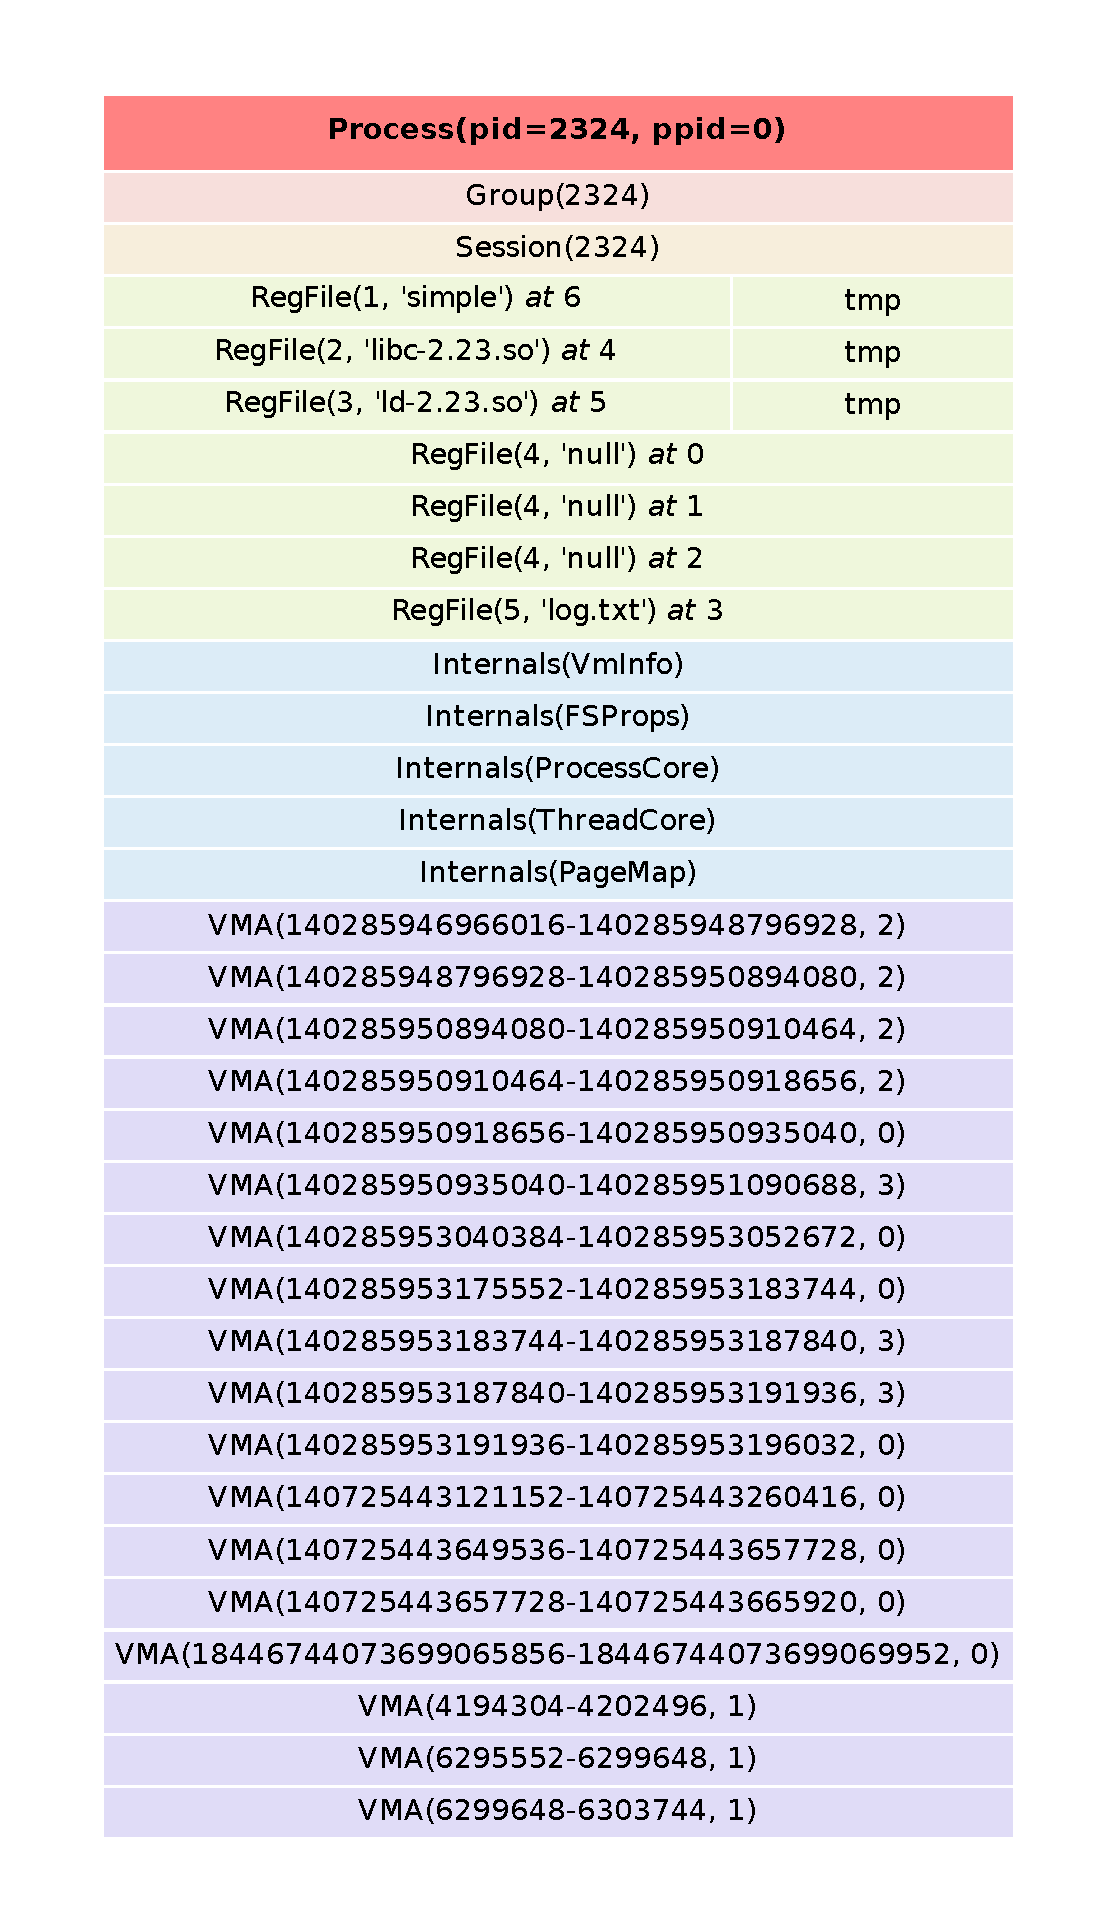
\includegraphics[width=\textwidth]{fig/exSimpleTree.pdf}
	\end{subfigure}
	\begin{subfigure}[b]{0.5\textwidth}
		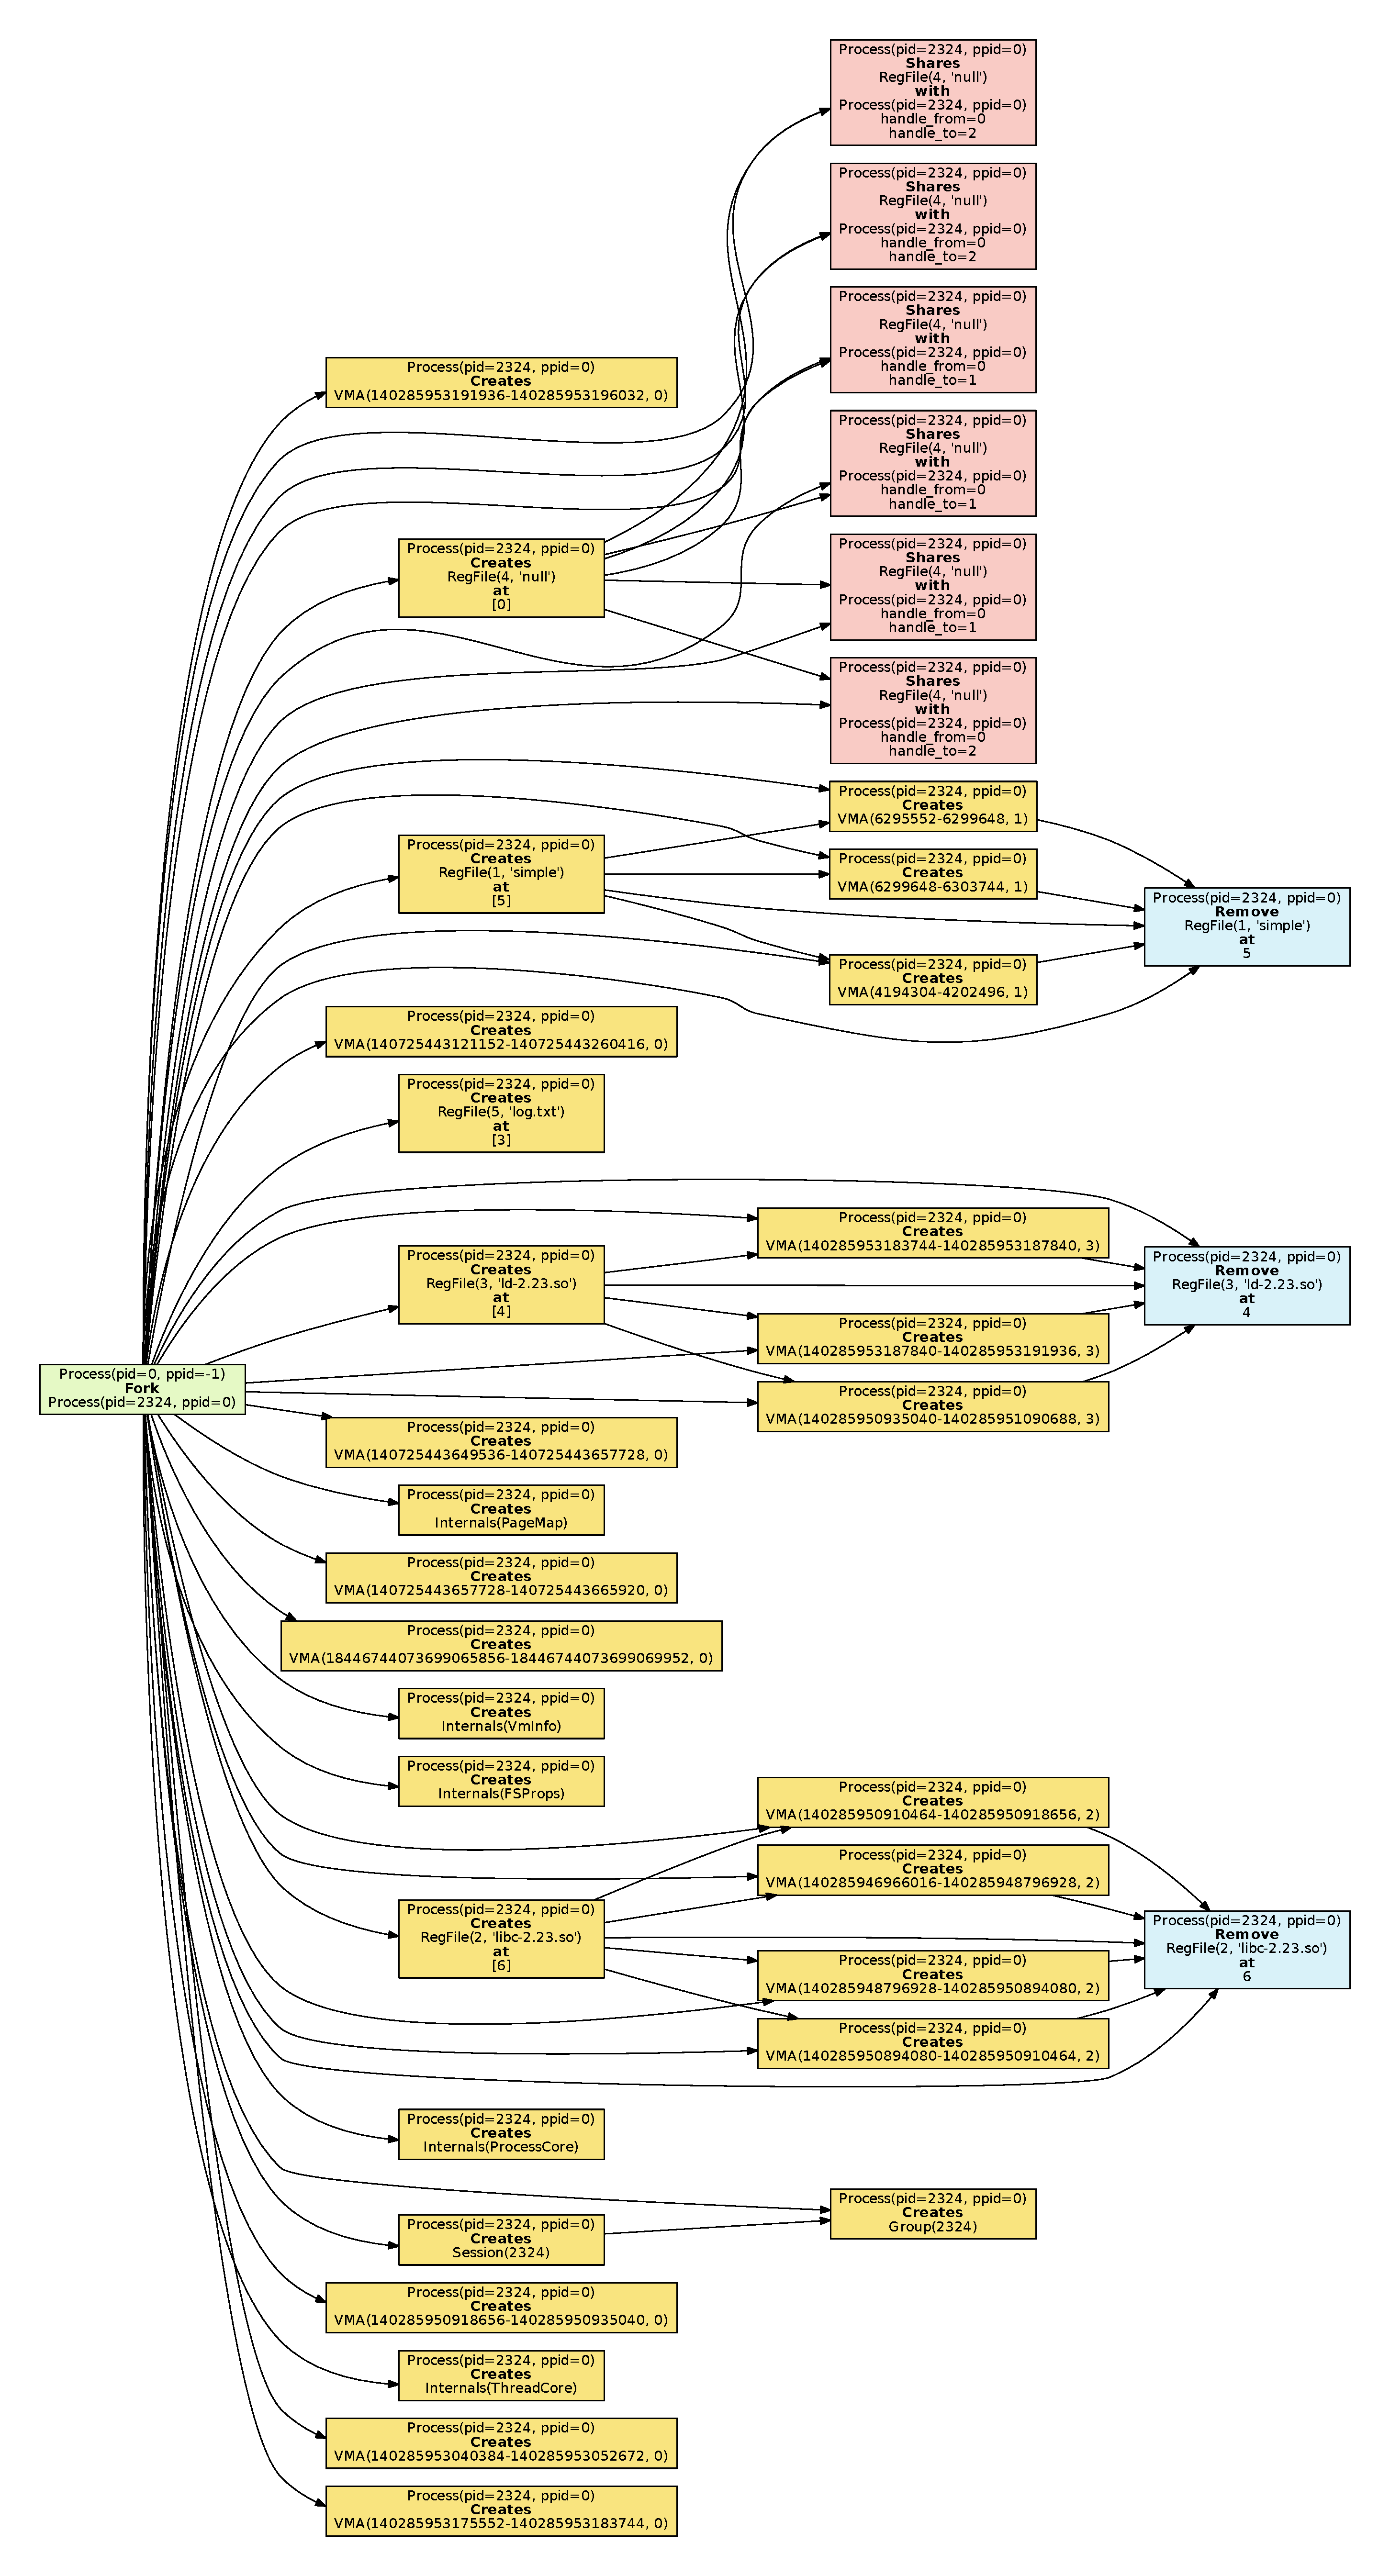
\includegraphics[width=\textwidth]{fig/exSimpleGraph.pdf}
	\end{subfigure}
	\caption{Дерево из одного процесса и граф действий восстановления для него}
	\label{chap2:fig:oneprocess}
\end{figure}

Граф действий с выстроенными рёбрами будет выглядеть для него так, как изображено справа на рисунке~\ref{chap2:fig:oneprocess}. Граф получается довольно большим, но структура этого графа проста и древесна. В полученном дереве лишь три уровня.

\subsection{Пример с группами}

Рассмотрим следующее дерево процессов, изображённую на рисунке~\ref{chap2:fig:groupspstree}. Это дерево идентично тому, которое использовалось в примере~\ref{chap1:exmp:criugroups}. И \texttt{criu} возвращает ошибку при попытке восстановить дерево из таких процессов. 


\begin{figure}[ht!]
	\centering
	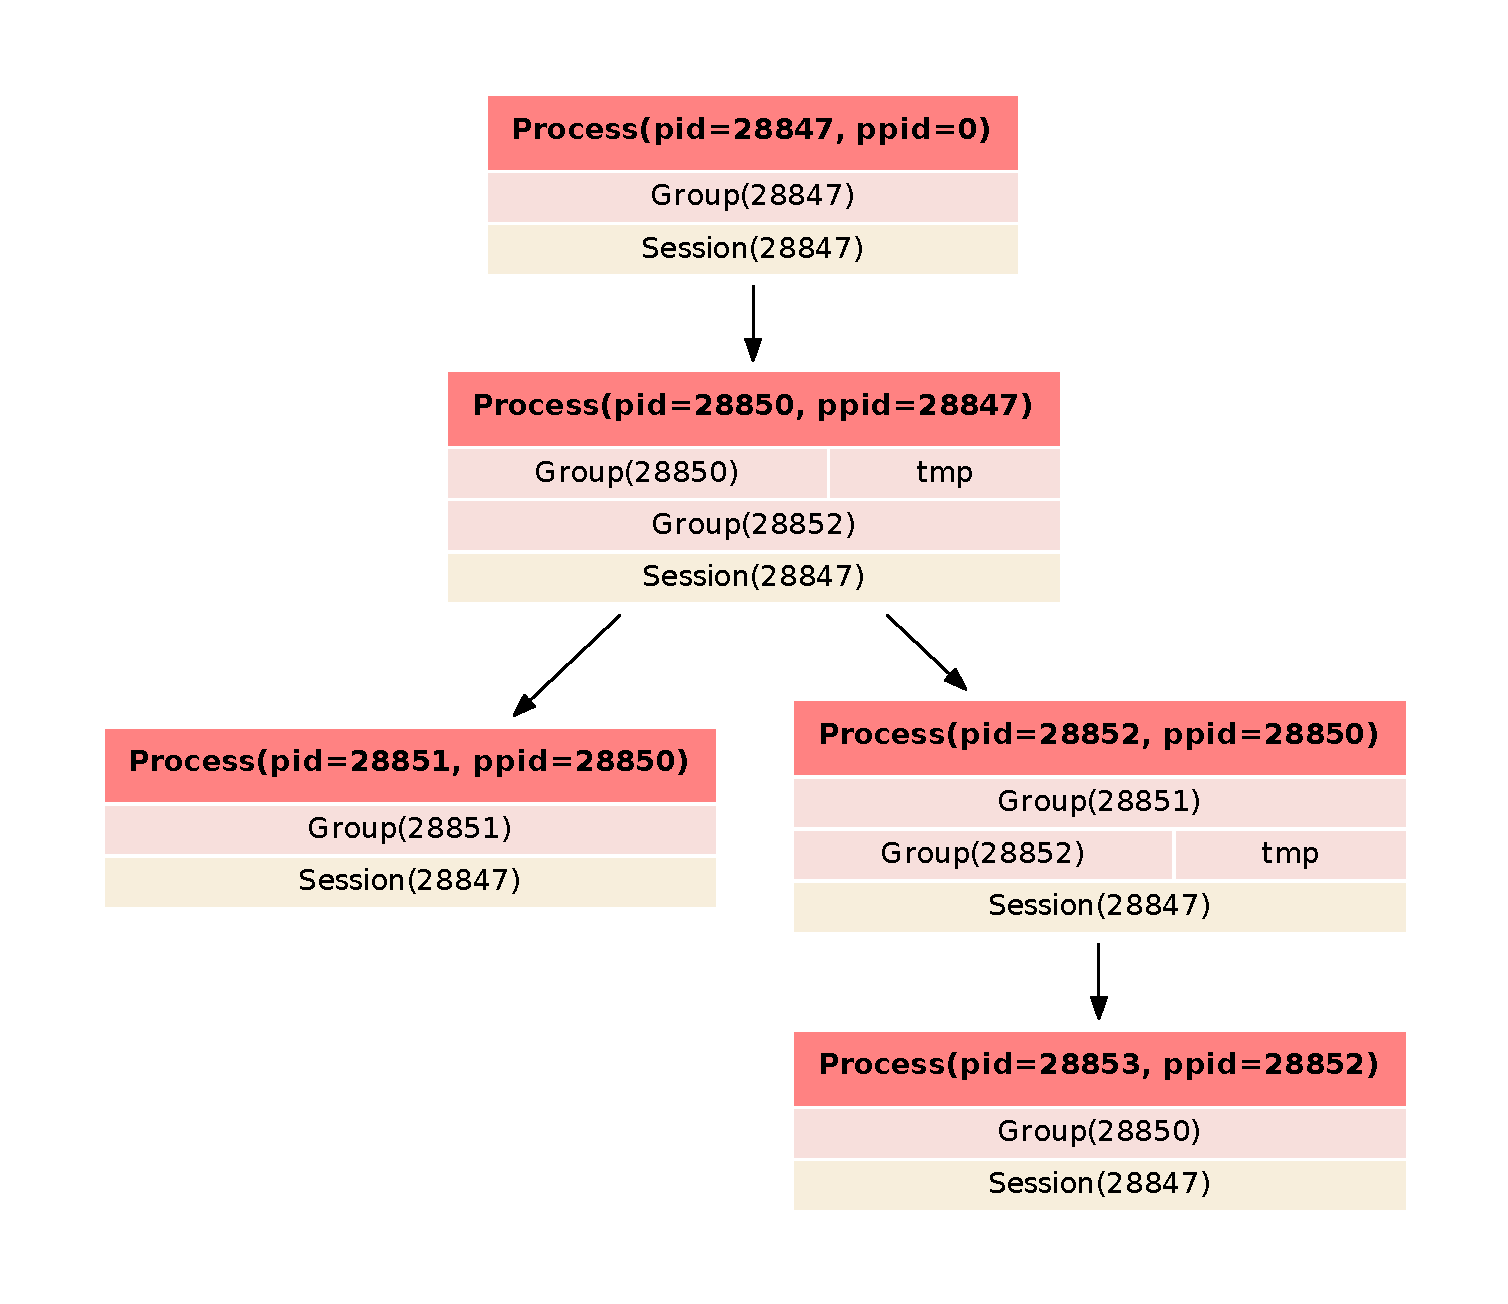
\includegraphics[scale=0.4]{fig/examplePstree.pdf}
\caption{Дерево для примера с группами}
\label{chap2:fig:groupspstree}
\end{figure}

После построения графа действий мы получаем граф, изображённый на рисунке~\ref{chap2:fig:groupsgraph}. Предложенный алгоритм строит ациклический граф и возвращает последовательность действий, изображённую на рисунке~\ref{chap2:fig:groupssorted}.



Полученная последовательность действий и граф хорошо показывают, что полученный алгоритм может разрешать довольно нетривиальные зависимости между ресурсами.

\begin{figure}[ht!]
	\begin{subfigure}[b]{0.7\textwidth}
		\centering
		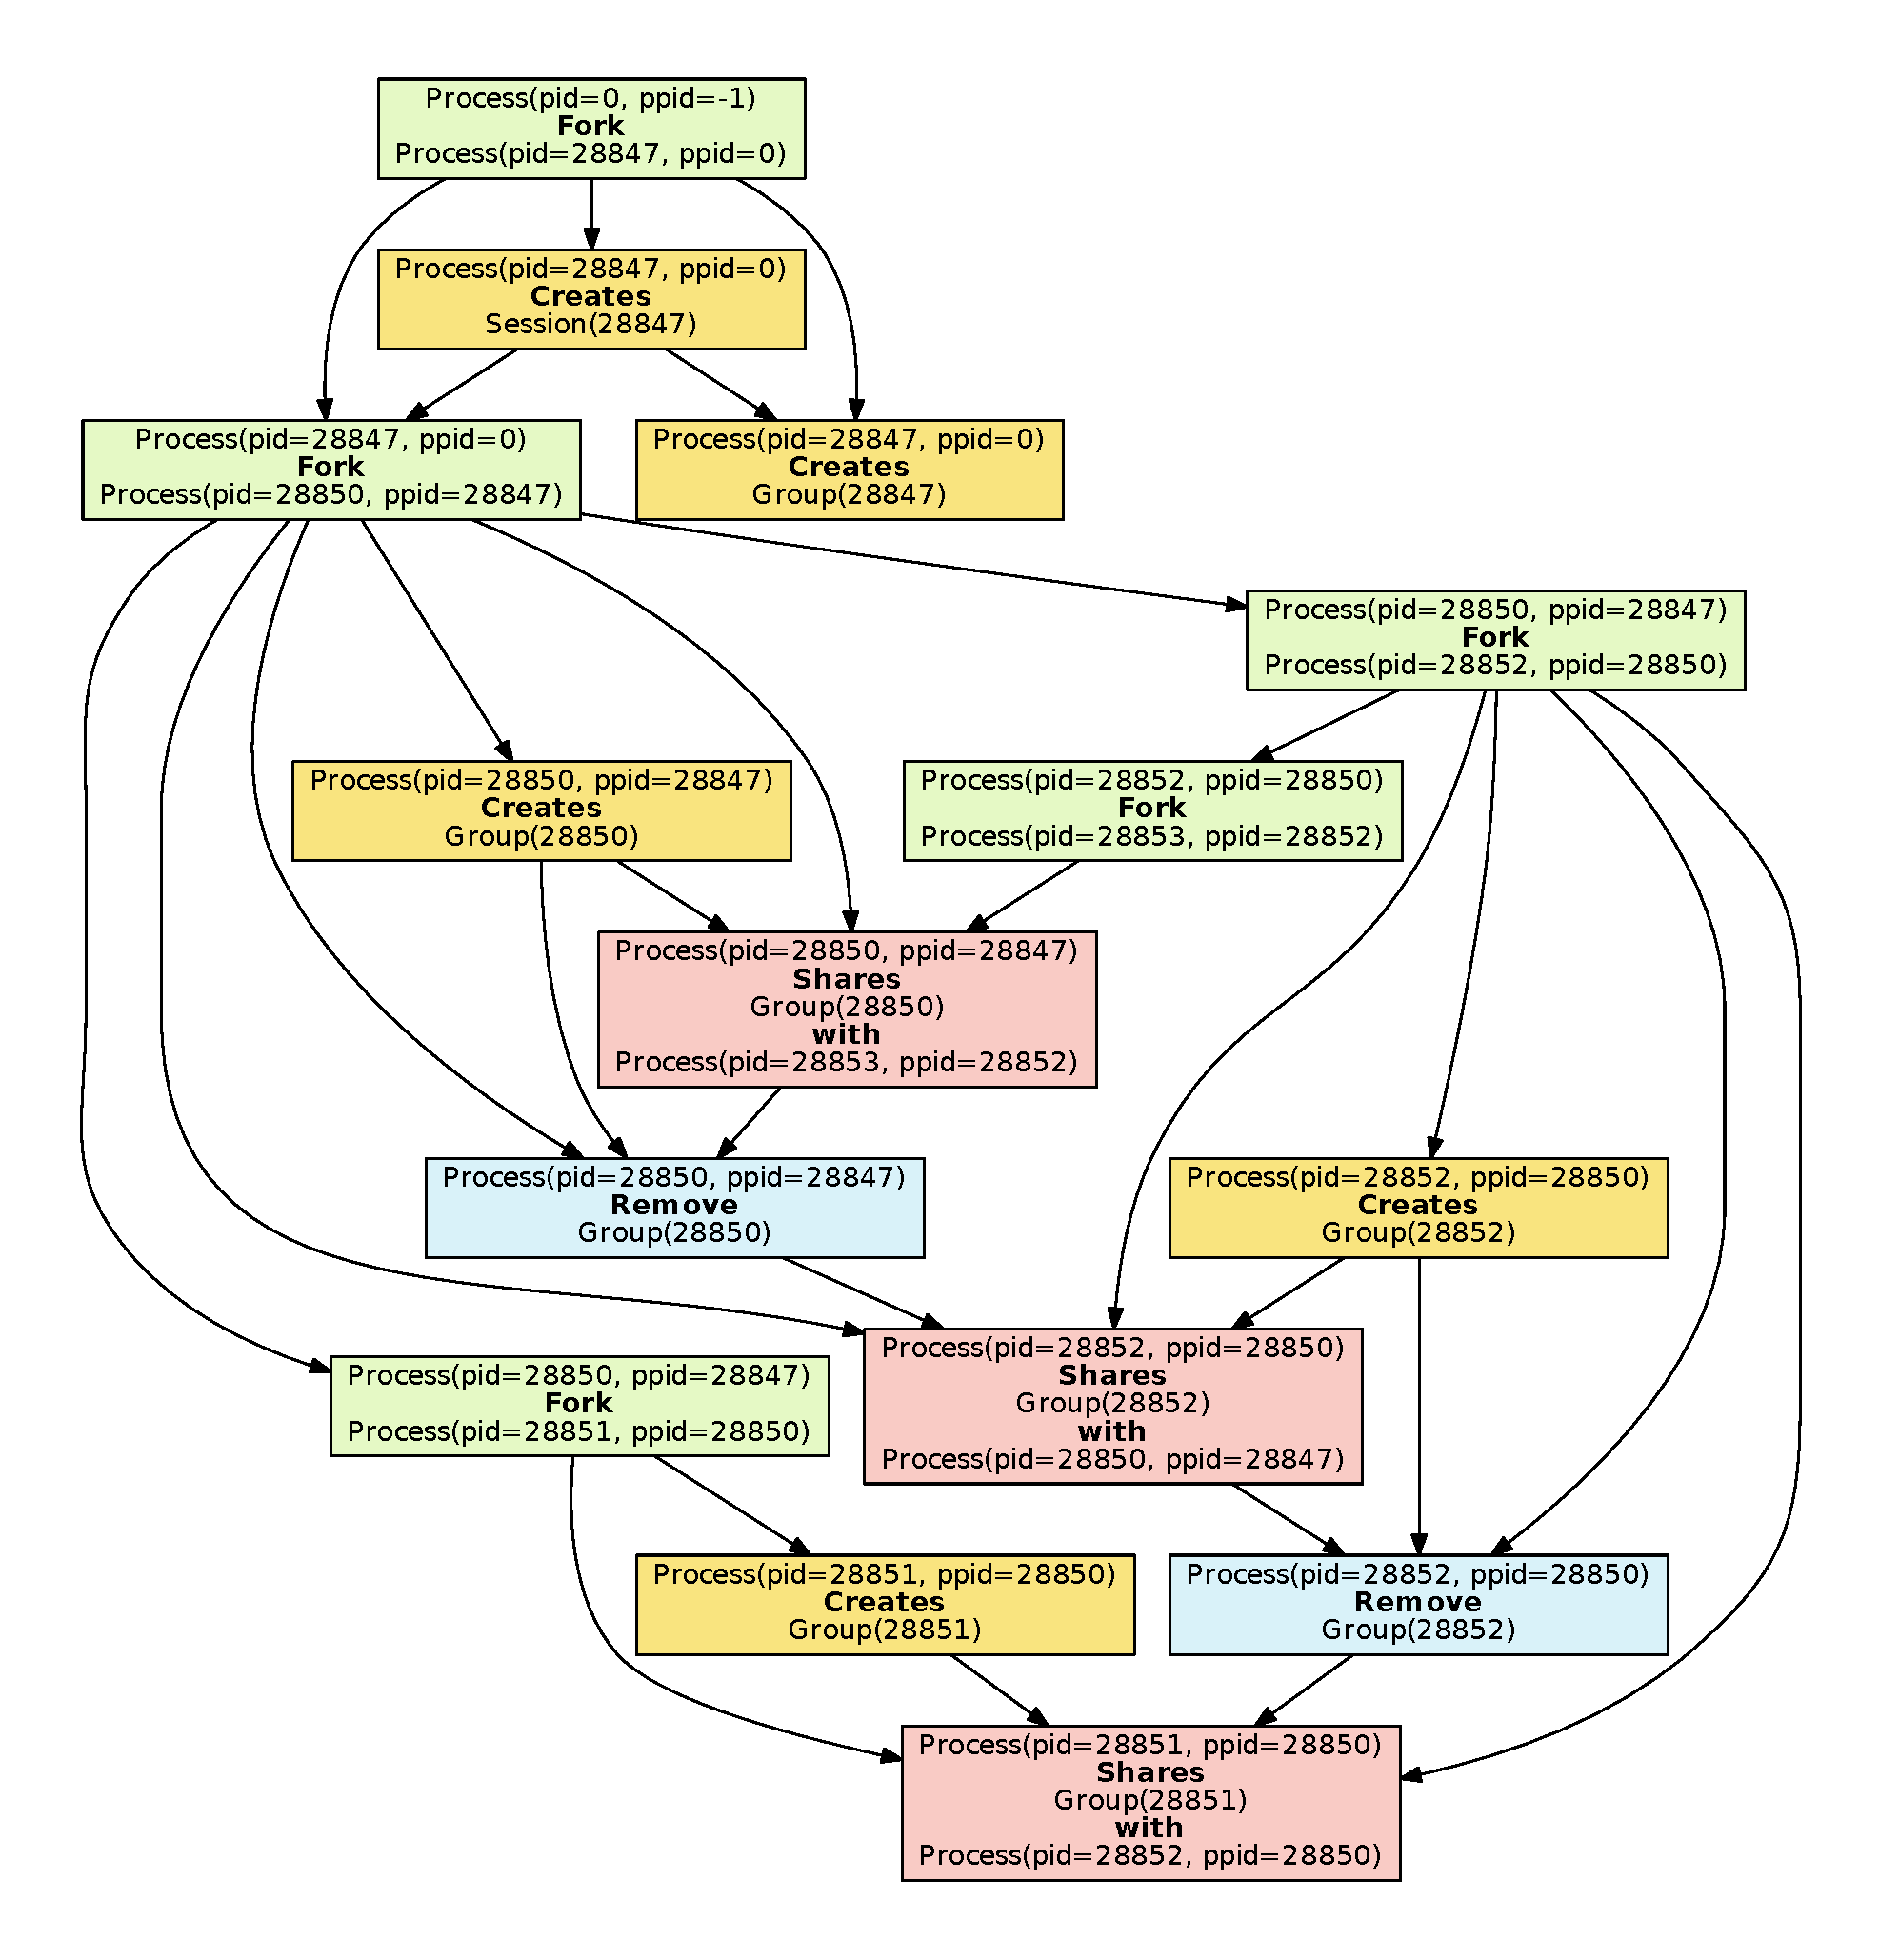
\includegraphics[width=\textwidth]{fig/exampleActGraph.pdf}
	\caption{Граф действий для примера}
	\label{chap2:fig:groupsgraph}
	\end{subfigure}
	\begin{subfigure}[b]{0.25\textwidth}
		\centering
		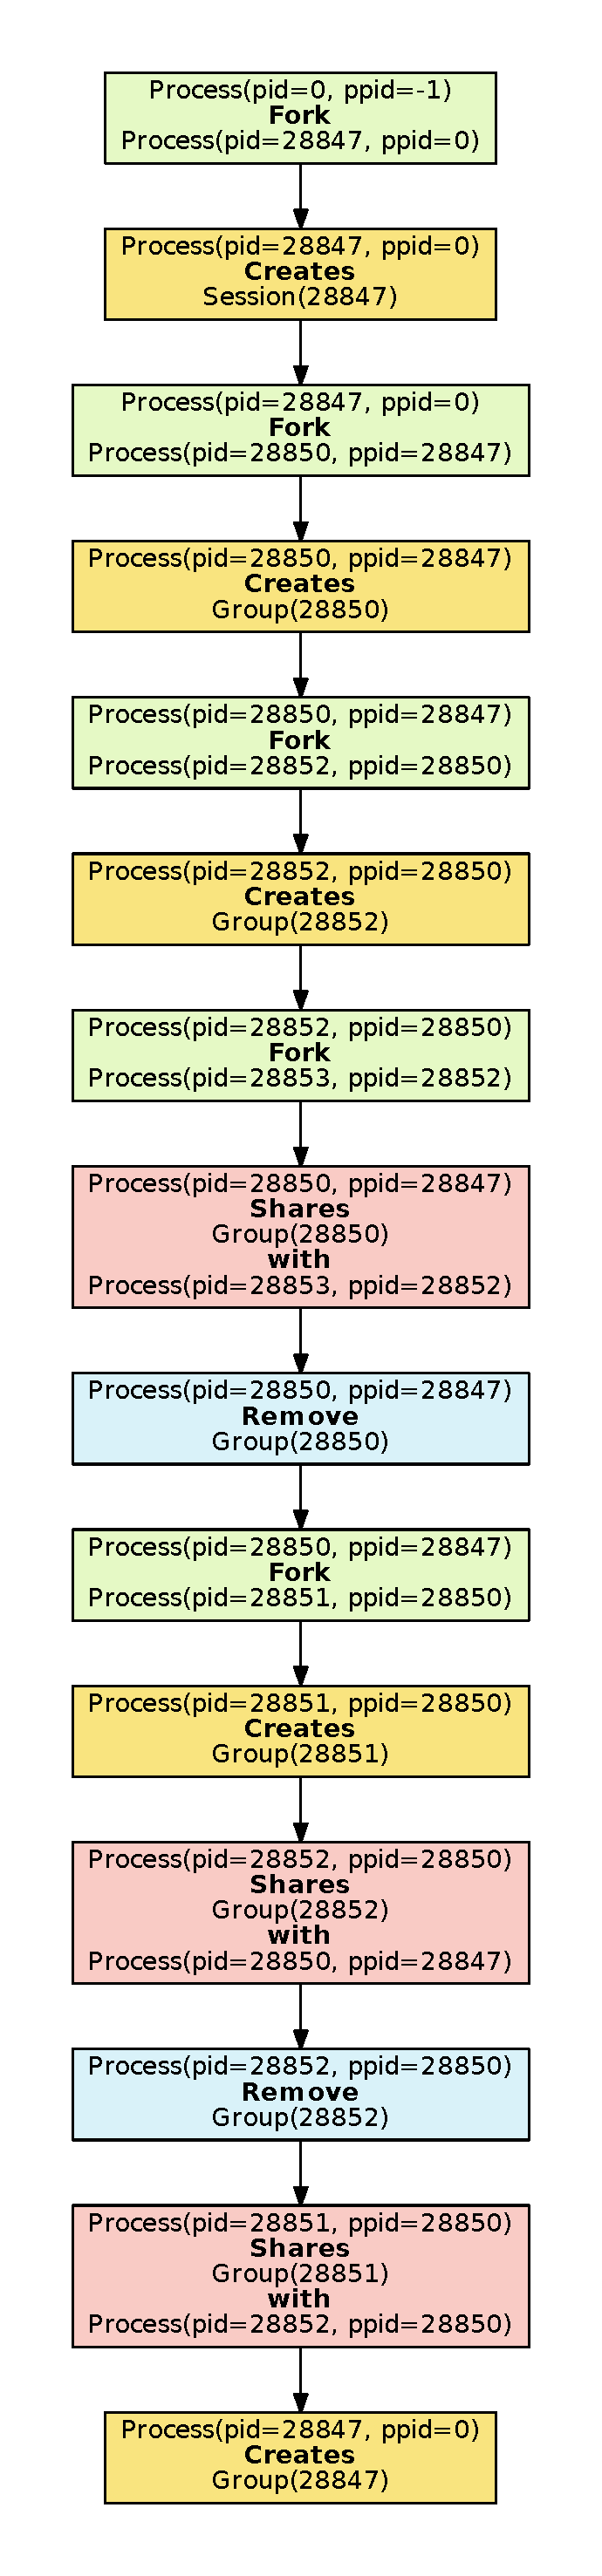
\includegraphics[width=\textwidth]{fig/exampleActSorted.pdf}
	\caption{Упорядоченная последовательность действий для примера с группами}
	\label{chap2:fig:groupssorted}
	\end{subfigure}
\end{figure}

\subsection{Цикличность графа действий}
\label{chap2:subsec:cycles}

Предложенный в этой работе подход является достаточно гибким для описания огромного числа зависимостей между ресурсами
и конфигураций процессов, но пока что он не способен восстановить абсолютно любое дерево процессов. Это связано с тем, что граф действий не всегда будет ациклическим.

Рассмотрим следующий пример дерева процессов, изображённый на рисунке~\ref{chap2:fig:imppstree}. В этом дереве мы видим
два процесса, которые обменялись группами (третий процесс, с ppid=0 является лидером всех сессии): 21650 и 21651. Поскольку текущий подход пытается создавать команды создания и разделения ресурсов, которые исполняются только теми процессами, которые присутствуют в дереве для восстановления, то данное дерево получается невозможным для восстановления, т.к. с одной стороны процесс 21650 должен создать группу 21650 и поделиться ею с 21651, причём так, что этот обмен будет последним действием, вовлекающим процесс 21651 в изменение группы (т.к. это конечная целевая группа для этого процесса). Но при этом то же самое должно произойти и со стороны процесса 21651. Эта ситуация наглядно проявляется в графе действий, который, вместе с возникающим циклом, изображён на рисунке

\begin{figure}[ht!]
	\centering
	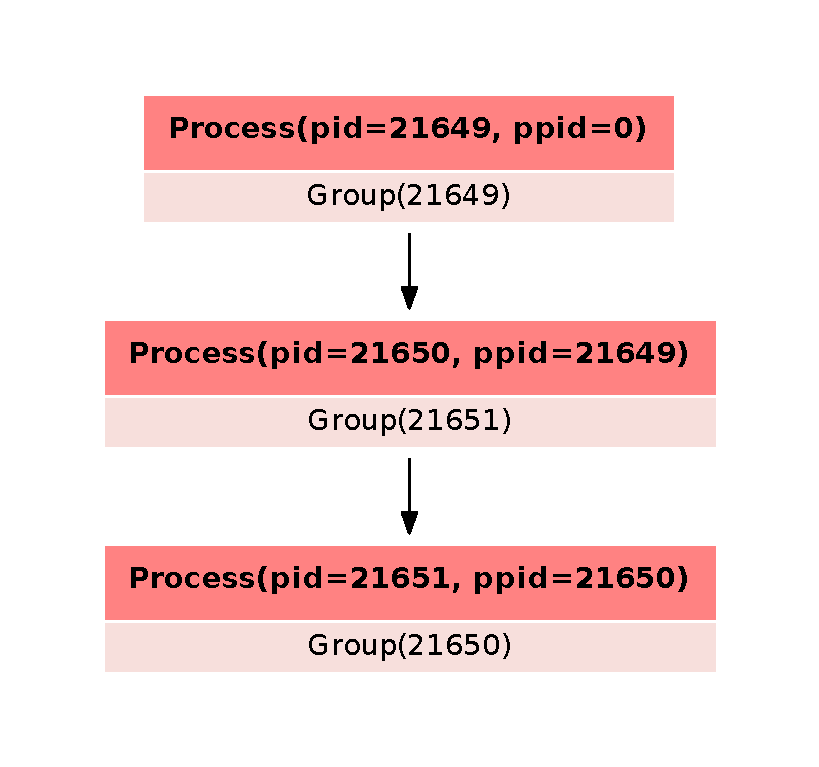
\includegraphics[scale=0.4]{fig/badextree.pdf}
\caption{Дерево, которое не восстановить в рамках текущей модели}
\label{chap2:fig:imppstree}
\end{figure}


\begin{figure}[ht!]
	\begin{subfigure}[b]{0.5\textwidth}
		\centering
		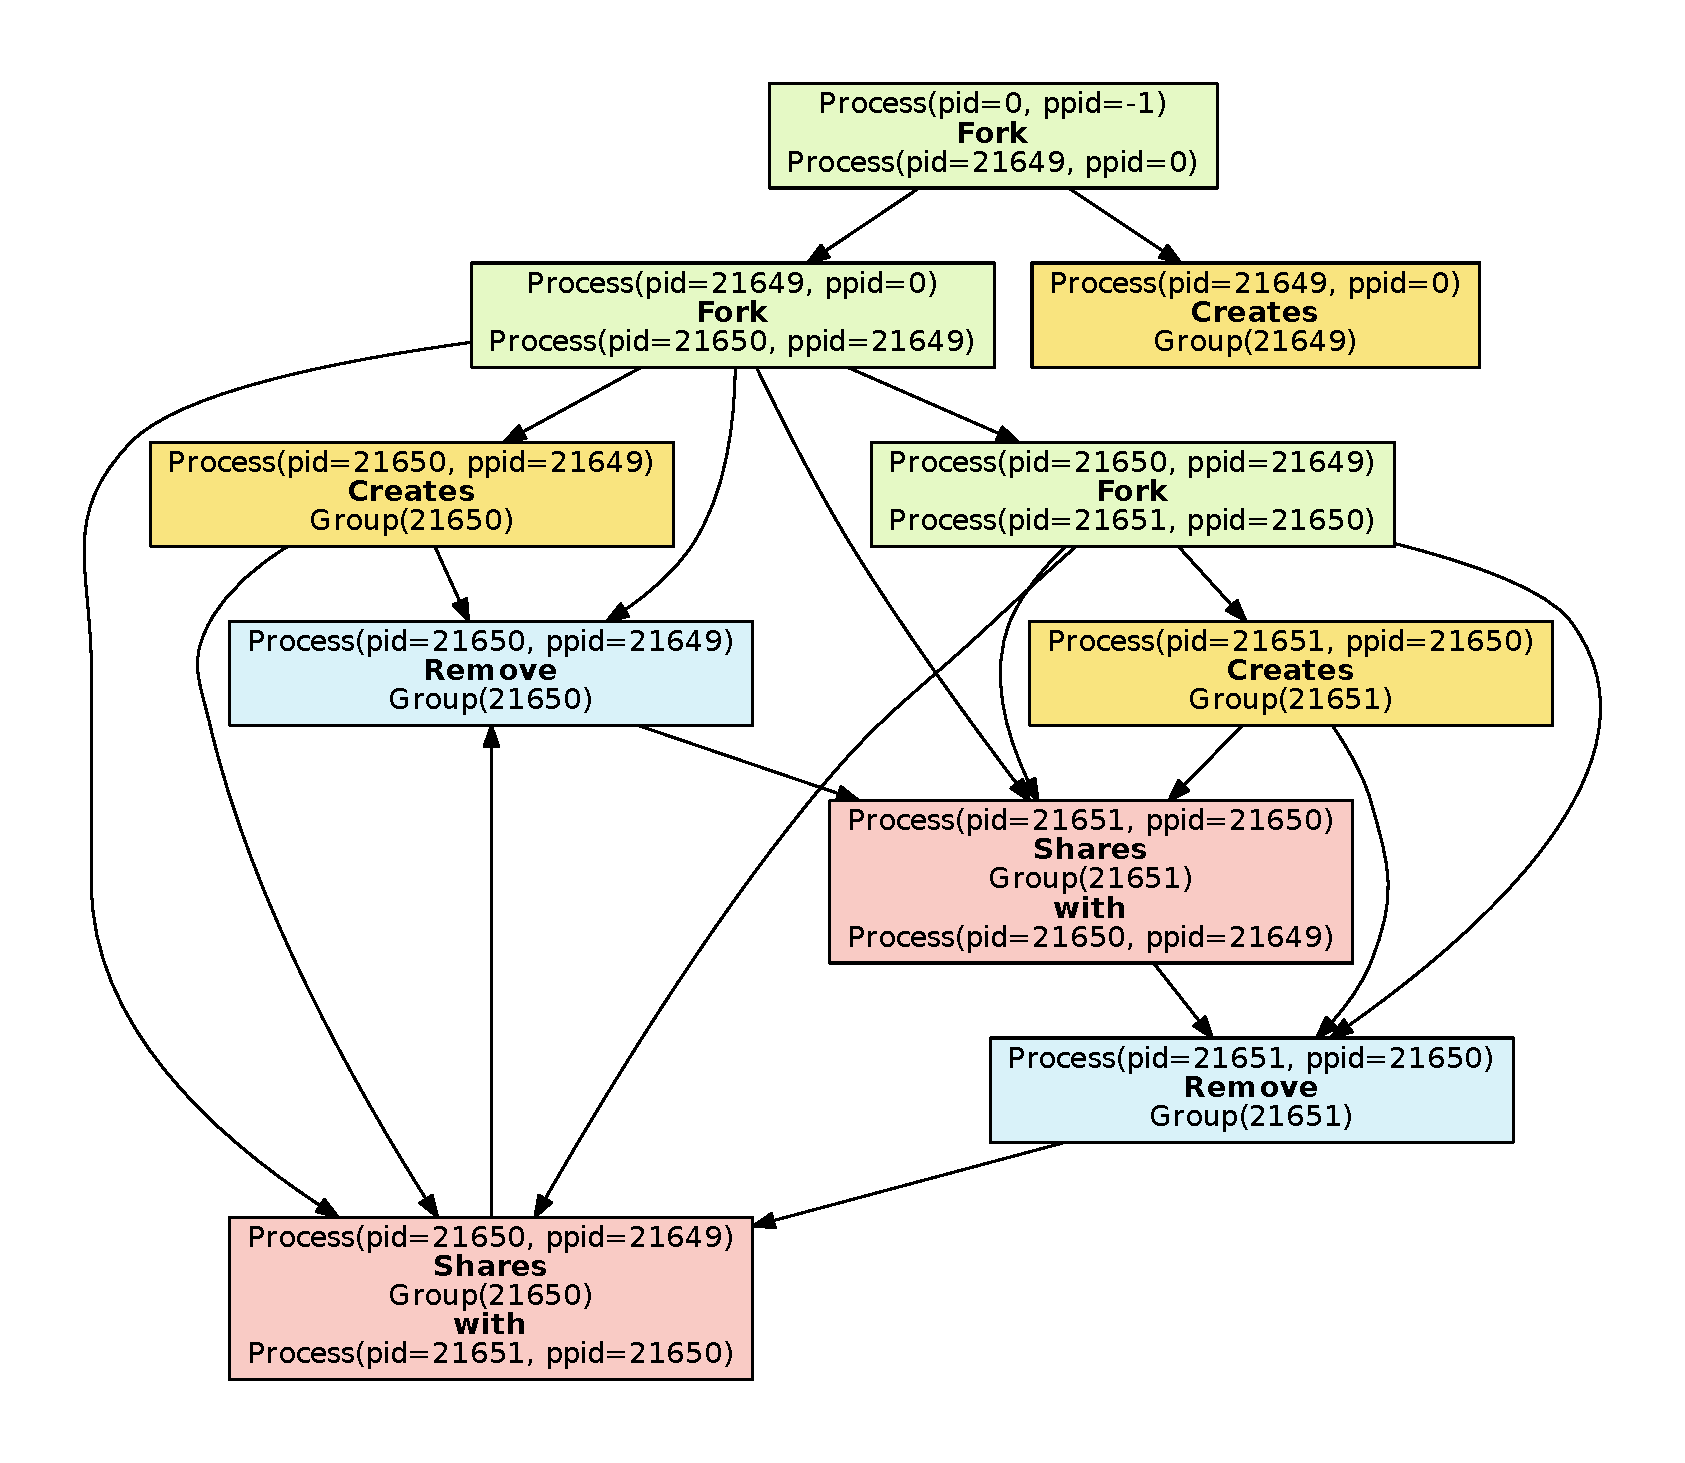
\includegraphics[width=\textwidth]{fig/badexgraph.pdf}
	\caption{Граф действий для примера с обменом конфликтующими}
	\label{chap2:fig:impgraph}
	\end{subfigure}
	\begin{subfigure}[b]{0.46\textwidth}
		\centering
		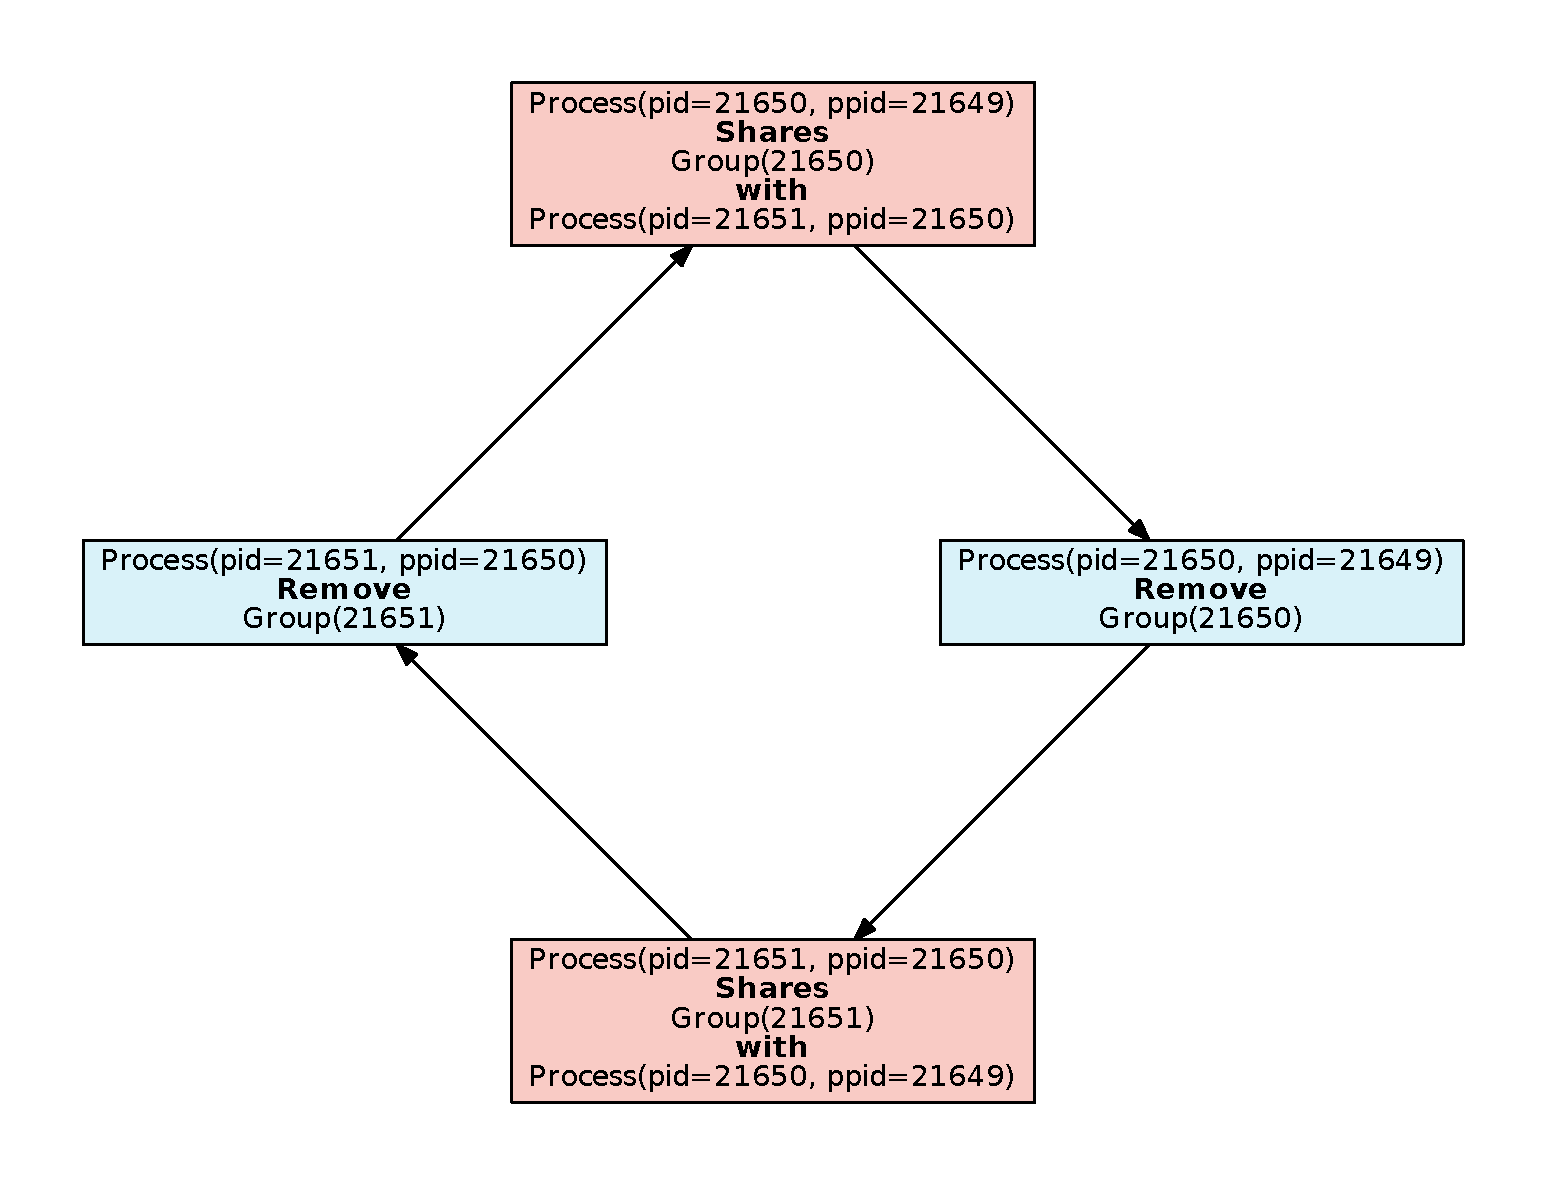
\includegraphics[width=\textwidth]{fig/badexcycle.pdf}
	\caption{Возникший цикл на действиях}
	\label{chap2:fig:impcycle}
	\end{subfigure}
\end{figure}

Такие циклы будут возникать каждый раз, когда в графе действий возникает ситуация циклического обмена конфликтующими между собой ресурсами. Одним из возможных способов решения этой проблемы является добавление вспомогательных процессов,
которые бы могли выступать <<третьим>> лицом, сохраняющим ресурс при обмене (можно провести аналогии с обменом значений двух переменных).

\section{Программная реализация генератора команд}

Генератор команд, реализованный в рамках данной работы, написан на языке \texttt{python}.

% \section{Классификация ресурсов}
% \label{chap2:seq:realres}
% TODO: тут будет информация про реальные ресурсы Linux, про то, какими свойствами они обладают в рамках приведённой модели.

% \subsection{Идентификаторы процесса}

% \begin{table}[ht!]
% \centering
% \begin{tabular}{|c|c|c|c|}
% 	\hline
% 	\textbf{Ресурс} & \textit{\textbf{handle}} & $\isinherited{r}$ & $\issharable{r}$ \\
% 	\hline
% 	\hline
% 	Сам процесс & pid & нет & нет \\
% 	\hline
% 	Группа процесса & pgid & да & да, \texttt{setpgid()} \\
% 	\hline
% 	Сессия процесса & ssid & да & нет \\
% 	\hline
% 	Идентификатор пользователя & uid & да & да, \texttt{setuid()} \\
% 	\hline
% \end{tabular}
% \end{table}
